% =====================================================================

%  Post-Quantum Cryptography for the Novice, the Enjoyer,
%  the Deployer and the Academic
%  BalCCon, Novi Sad
%  Lena Heimberger
%
%  latexmk -pdf pqc-balccon.tex
%  Swap \usetheme{metropolis} for \usetheme{isec} to use your own theme;
%  the deck only relies on frametitle, standout frames and section pages.
% =====================================================================
\documentclass[aspectratio=169]{beamer}

\usetheme[progressbar=frametitle,numbering=fraction,block=fill]{metropolis}

\usepackage[utf8]{inputenc}
\usepackage[english]{babel}
\usepackage{amsmath,amssymb}
\usepackage{booktabs}
\usepackage{soul}
\usepackage{tikz}
\usepackage{tikzpeople}
\usepackage{pgfplots}
\pgfplotsset{compat=1.18}
\usetikzlibrary{arrows.meta,positioning,calc,fit,decorations.pathmorphing,
                shapes.geometric,backgrounds}

% ---- palette ---------------------------------------------------------
\definecolor{ink}{HTML}{2E2038}    % deep plum, body text + standout bg
\definecolor{pink}{HTML}{C13584}   % pink, primary accent
\definecolor{rose}{HTML}{F06FB0}   % light pink, fills and second series
\definecolor{blush}{HTML}{FFF7FC}  % near-white pink, slide background
\definecolor{peri}{HTML}{6C7BE0}   % periwinkle, diagrams and structure
\definecolor{sky}{HTML}{62B6E8}    % sky blue, third series
\definecolor{teal}{HTML}{1FA89B}   % the positive colour
\definecolor{coral}{HTML}{F4633A}  % the negative colour
\definecolor{gold}{HTML}{F5B23D}   % highlight, progress bar
\definecolor{mauve}{HTML}{9B8AA6}  % muted text, axes, grid

% keep the old role names so nothing else in the deck has to change
\colorlet{acc}{pink}
\colorlet{warm}{gold}
\colorlet{good}{teal}
\colorlet{bad}{coral}
\colorlet{grey}{mauve}
\colorlet{mBGcol}{blush}

\setbeamercolor{normal text}{fg=ink,bg=blush}
\setbeamercolor{alerted text}{fg=pink}
\setbeamercolor{frametitle}{bg=pink,fg=blush}
\setbeamercolor{progress bar}{fg=gold}
\setbeamercolor{progress bar in head/foot}{fg=rose}
\setbeamercolor{progress bar in section page}{fg=pink}
\setbeamercolor{block title}{bg=peri!12,fg=peri}
\setbeamercolor{block title alerted}{bg=pink!12,fg=pink}
\setbeamercolor{block body}{bg=blush}
\setbeamercolor{title separator}{fg=pink}
\setbeamercolor{itemize item}{fg=pink}
\setbeamercolor{itemize subitem}{fg=peri}
% % ---- colours ---------------------------------------------------------
% \definecolor{mBGcol}{HTML}{fafafa}
% \definecolor{acc}{HTML}{6A5ACD}   % your purple
% \definecolor{warm}{HTML}{EB811B}
% \definecolor{good}{HTML}{2E7D32}
% \definecolor{bad}{HTML}{C62828}
% \definecolor{grey}{HTML}{9E9E9E}
% \definecolor{pink}{HTML}{C13584}
% % plain colour names for tikzpeople (it cannot take a!b expressions)
% \colorlet{shirtA}{acc!60}
% \colorlet{rose}{warm!70}
% \colorlet{teal}{good!60}
% \colorlet{blush}{acc}
% 
% \setbeamercolor{normal text}{bg=mBGcol}
% \setbeamercolor{alerted text}{fg=acc}
% \setbeamercolor{progress bar}{fg=warm}
% \setbeamercolor{block title alerted}{bg=acc!18,fg=acc}
% \setbeamercolor{block title}{bg=acc!10}
% 
\newcommand{\cgood}[1]{\textcolor{peri}{#1}}
\newcommand{\cbad}[1]{\textcolor{rose}{#1}}
\newcommand{\cwarm}[1]{\textcolor{teal}{#1}}
\newcommand{\cacc}[1]{\textcolor{pink}{#1}}
\newcommand{\cgrey}[1]{\textcolor{grey}{#1}}

% ---- one style for the four character slides -------------------------
\tikzset{
  hero/.style={minimum size=3.4cm},
}
\newcommand{\heroframe}[3]{% #1 = tikz person code, #2 = who, #3 = question
  \begin{frame}[plain]
    \centering
    \begin{tikzpicture}
      #1
    \end{tikzpicture}\\[0.6em]
    {\large\textbf{#2}}\\[0.4em]
    {\Large\cacc{\textit{``#3''}}}
  \end{frame}}

\title{Post-Quantum Cryptography}
\subtitle{for the Novice, the Enjoyer, the Deployer and the Academic}
\author{Lena Heimberger}
\date{BalCCon 2026, Novi Sad}

\begin{document}

\maketitle

% =====================================================================

\begin{frame}{Cryptography is already a part of your life}
  \centering
  
\begin{tikzpicture}[x=1cm,y=1cm,font=\scriptsize,
      lab/.style={anchor=north,grey,font=\scriptsize}]

    % message bubble
    \begin{scope}[shift={(0,0)}]
      \draw[acc,line width=1pt,fill=acc!10,rounded corners=4pt]
        (-0.75,-0.45) rectangle (0.75,0.55);
      \draw[acc,line width=1pt,fill=acc!10]
        (-0.35,-0.45) -- (-0.15,-0.8) -- (0.05,-0.45) -- cycle;
      \draw[acc!60,line width=1pt,line cap=round] (-0.45,0.25) -- (0.45,0.25);
      \draw[acc!60,line width=1pt,line cap=round] (-0.45,-0.05) -- (0.2,-0.05);
      \node[lab] at (0,-1.05) {messages};
    \end{scope}

    \uncover<2->{
    % contactless card
    \begin{scope}[shift={(2.8,0)}]
      \draw[peri,line width=1pt,fill=peri!10,rounded corners=3pt]
        (-0.85,-0.5) rectangle (0.55,0.45);
      \draw[peri!70,line width=1pt,fill=warm!50,rounded corners=1pt]
        (-0.65,-0.05) rectangle (-0.3,0.2);
      \foreach \r in {0.22,0.38,0.54}{
        \draw[peri,line width=0.9pt] (0.15,-0.03) ++(-40:\r) arc (-40:40:\r);}
      \node[lab] at (-0.15,-1.05) {payments};
    \end{scope}
  }

    % car key
    \uncover<3->{
    \begin{scope}[shift={(5.6,0)}]
      \draw[good,line width=1pt,fill=good!10,rounded corners=4pt]
        (-0.4,-0.55) rectangle (0.4,0.45);
      \fill[good] (0,0.05) circle (0.13);
      \foreach \r in {0.3,0.45}{
        \draw[good!70,line width=0.9pt] (0,0.05) ++(50:\r) arc (50:130:\r);}
      \node[lab] at (0,-1.05) {your car};
    \end{scope}
  }

    % passport
    \uncover<4->{
    \begin{scope}[shift={(8.4,0)}]
      \draw[warm,line width=1pt,fill=warm!12,rounded corners=3pt]
        (-0.5,-0.6) rectangle (0.5,0.55);
      \draw[warm!80,line width=0.9pt] (0,0.15) circle (0.22);
      \draw[warm!80,line width=0.9pt] (-0.3,-0.25) -- (0.3,-0.25);
      \node[lab] at (0,-1.05) {your ID};
    \end{scope}
  }

    % wifi
    \uncover<5->{
    \begin{scope}[shift={(11.0,0)}]
      \fill[rose] (0,-0.45) circle (0.1);
      \foreach \r in {0.3,0.5,0.7}{
        \draw[rose,line width=1pt] (0,-0.45) ++(35:\r) arc (35:145:\r);}
      \node[lab] at (0,-1.05) {every connection};
    \end{scope}
  }
  \end{tikzpicture}
  \vspace{4mm}
  \begin{itemize}
    \item<6-> All of the cryptography is
      being replaced in the next ten years.
    \item<7-> Touches an \cacc{lot} of code.
    \item<8-> \cacc{Math is too complicated for me} \\ \pause
      It's a skillset, not a seperate function. 
  \end{itemize}
\end{frame}

\begin{frame}{Mosca's inequality: How long until my secret is revealed? }
  \vspace{2em}
  \centering

  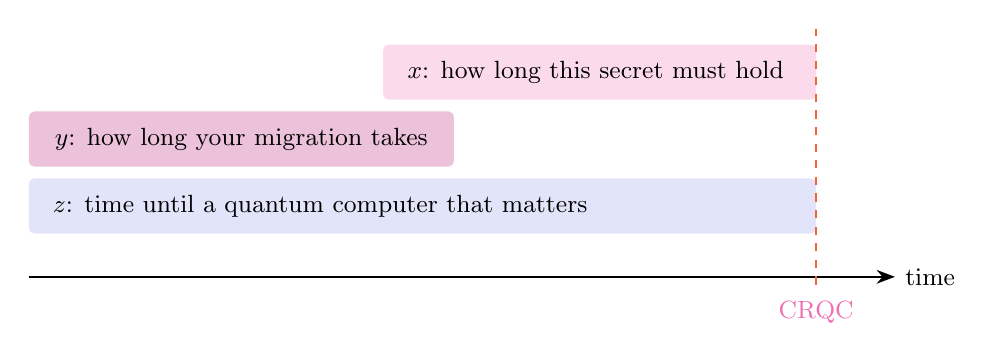
\begin{tikzpicture}[font=\small,x=1cm,y=1cm]
    \uncover<2->{
    \fill[rose!25,rounded corners=2pt]  (4.5,1.7) rectangle (10,2.4);
    \node at (7.2,2.05) {$x$: how long this secret must hold};
  }
    \uncover<3->{
    \fill[pink!30,rounded corners=2pt]  (0,0.85) rectangle (5.4,1.55);
    \node at (2.7,1.2) {$y$: how long your migration takes};
  }
    \uncover<4->{
    \fill[peri!20,rounded corners=2pt]   (0,0) rectangle (10,0.7);
    \node at (3.7,0.35) {$z$: time until a quantum computer that matters};
    \draw[-{Stealth},thick] (0,-0.55) -- (11,-0.55) node[right]{time};
    \draw[bad,thick,dashed] (10,-0.65) -- (10,2.6);
    \node at (10,-1) { \cbad{CRQC}};
  }
  \end{tikzpicture}
    \uncover<5->{
  \begin{center}
    \cacc{\Large If $x + y > z$, you are already too late.}
  \end{center}
  \vfill
  \footnotesize\cgrey{M. Mosca. \emph{Cybersecurity in an Era with Quantum
  Computers: Will We Be Ready?} IEEE Security \& Privacy 16(5), 2018.}
}


\end{frame}

\begin{frame}{Where are we? }
  \vspace{-3em}
  \begin{figure}
    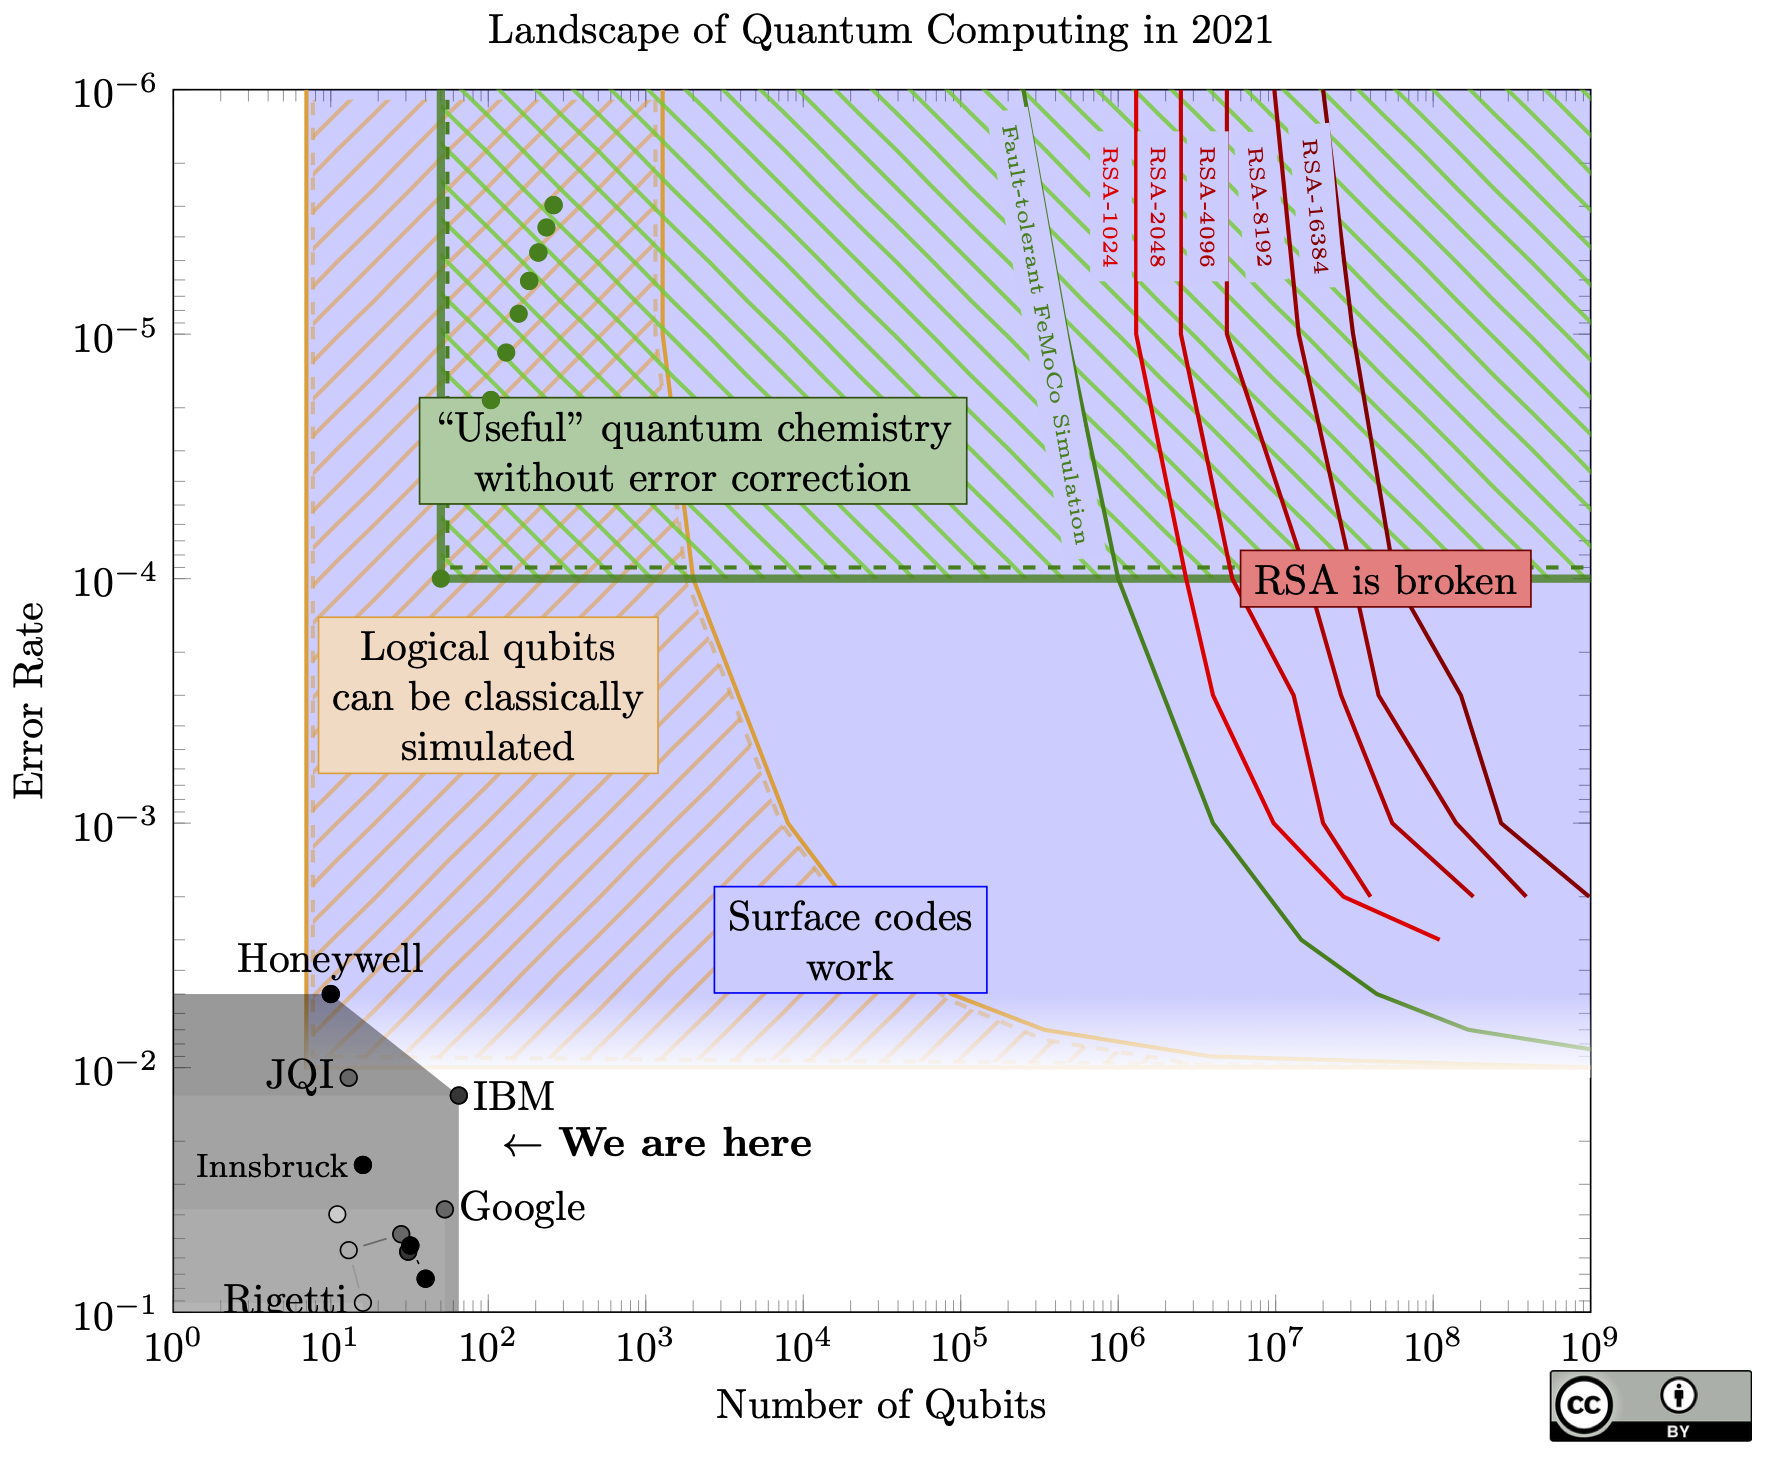
\includegraphics[scale=0.15]{figures/quantum-diagram-2021-new.png}
    \caption{\scriptsize\url{https://sam-jaques.appspot.com/quantum\_landscape}}
  \end{figure}
\end{frame}

\begin{frame}{Where are we? }
  \vspace{-3em}
  \begin{figure}
    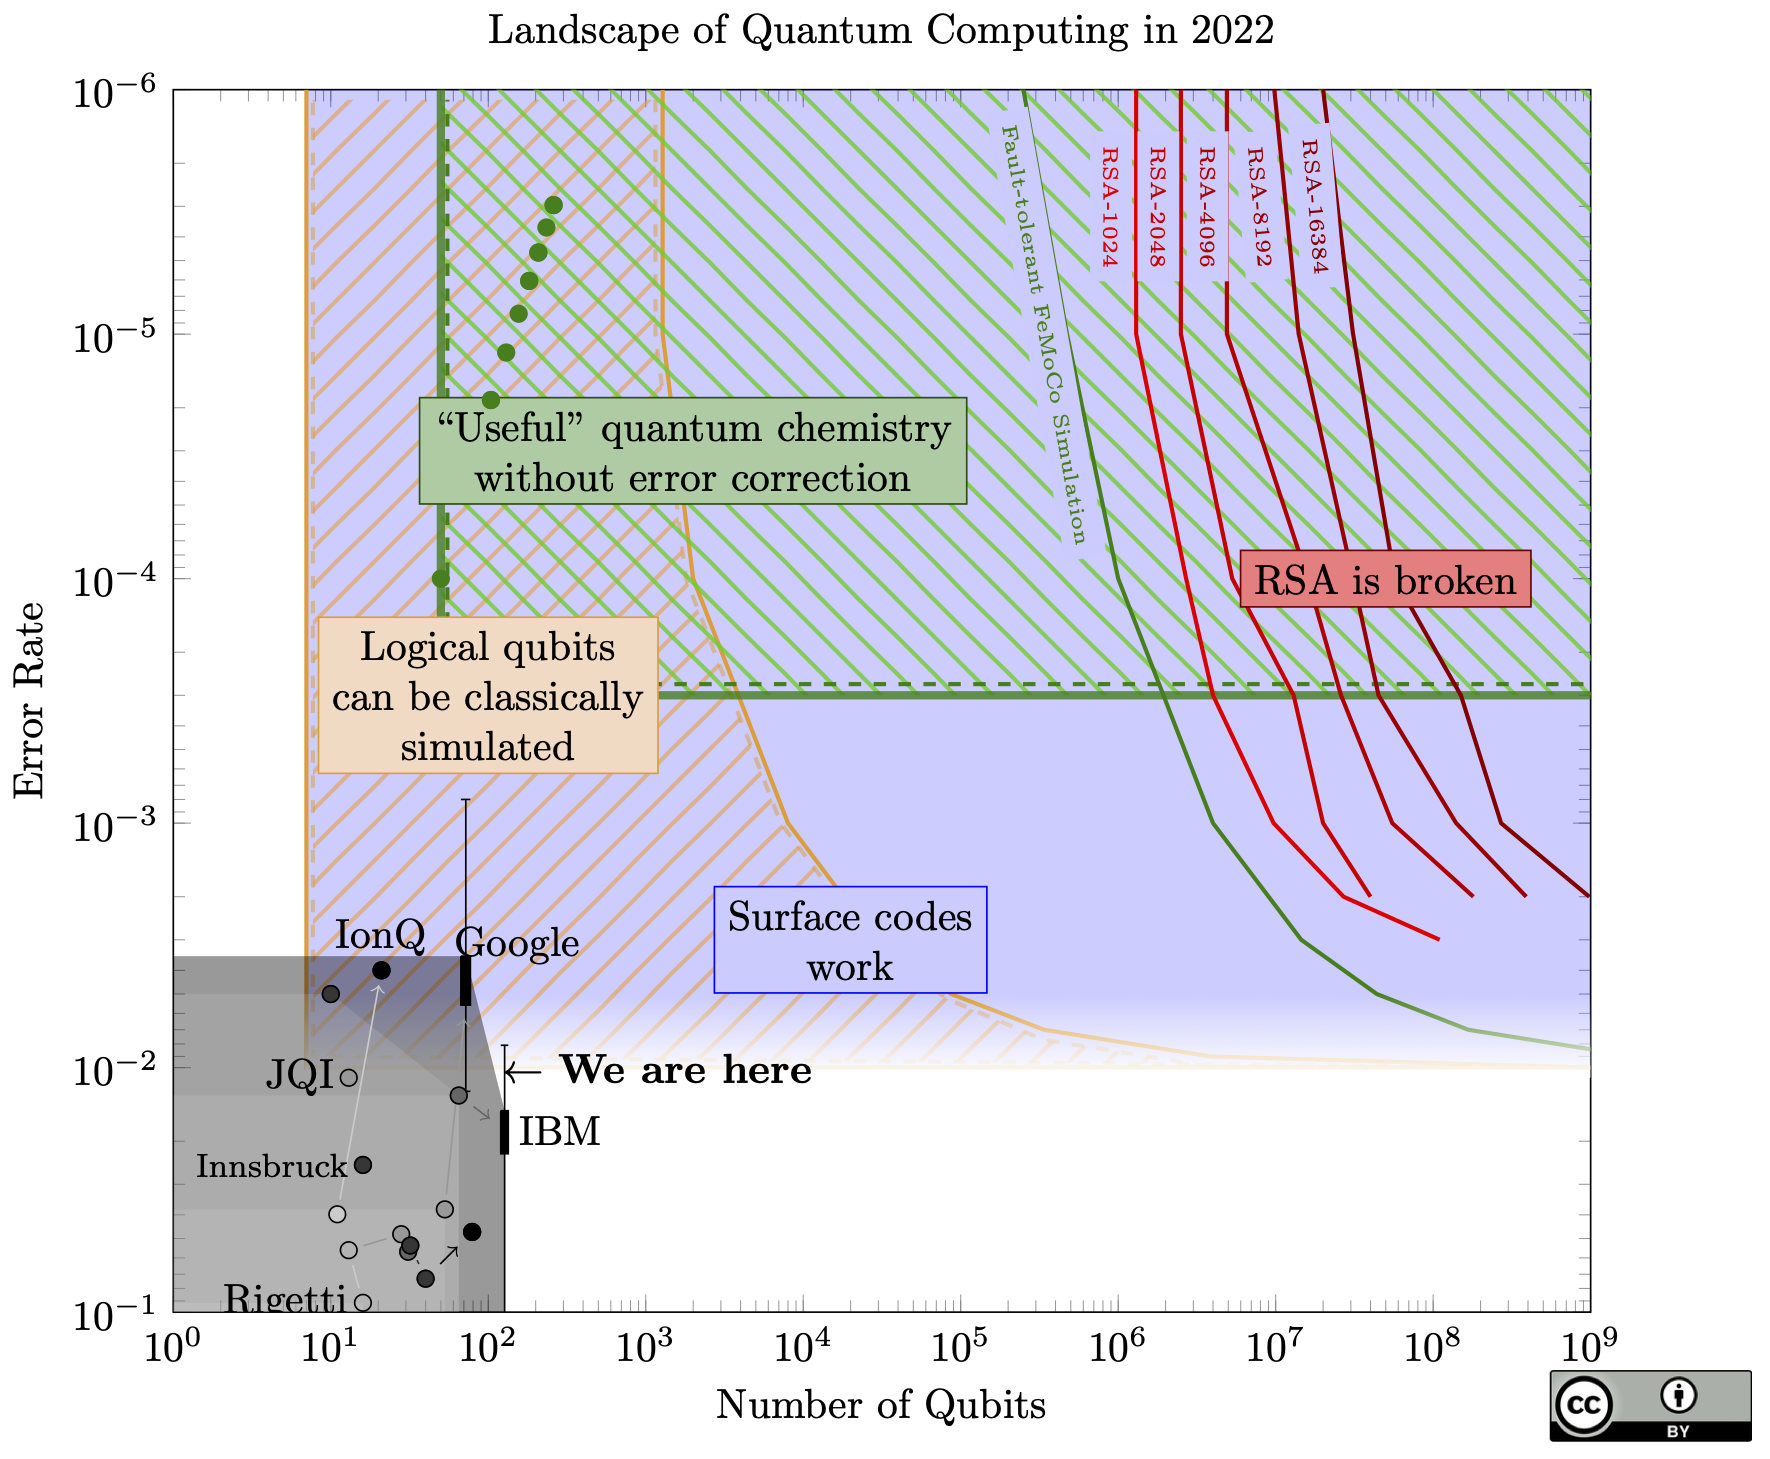
\includegraphics[scale=0.15]{figures/quantum-diagram-2022-new.png}
    \caption{\scriptsize\url{https://sam-jaques.appspot.com/quantum\_landscape}}
  \end{figure}
\end{frame}

 \begin{frame}{Where are we? }
   \vspace{-3em}
   \begin{figure}
     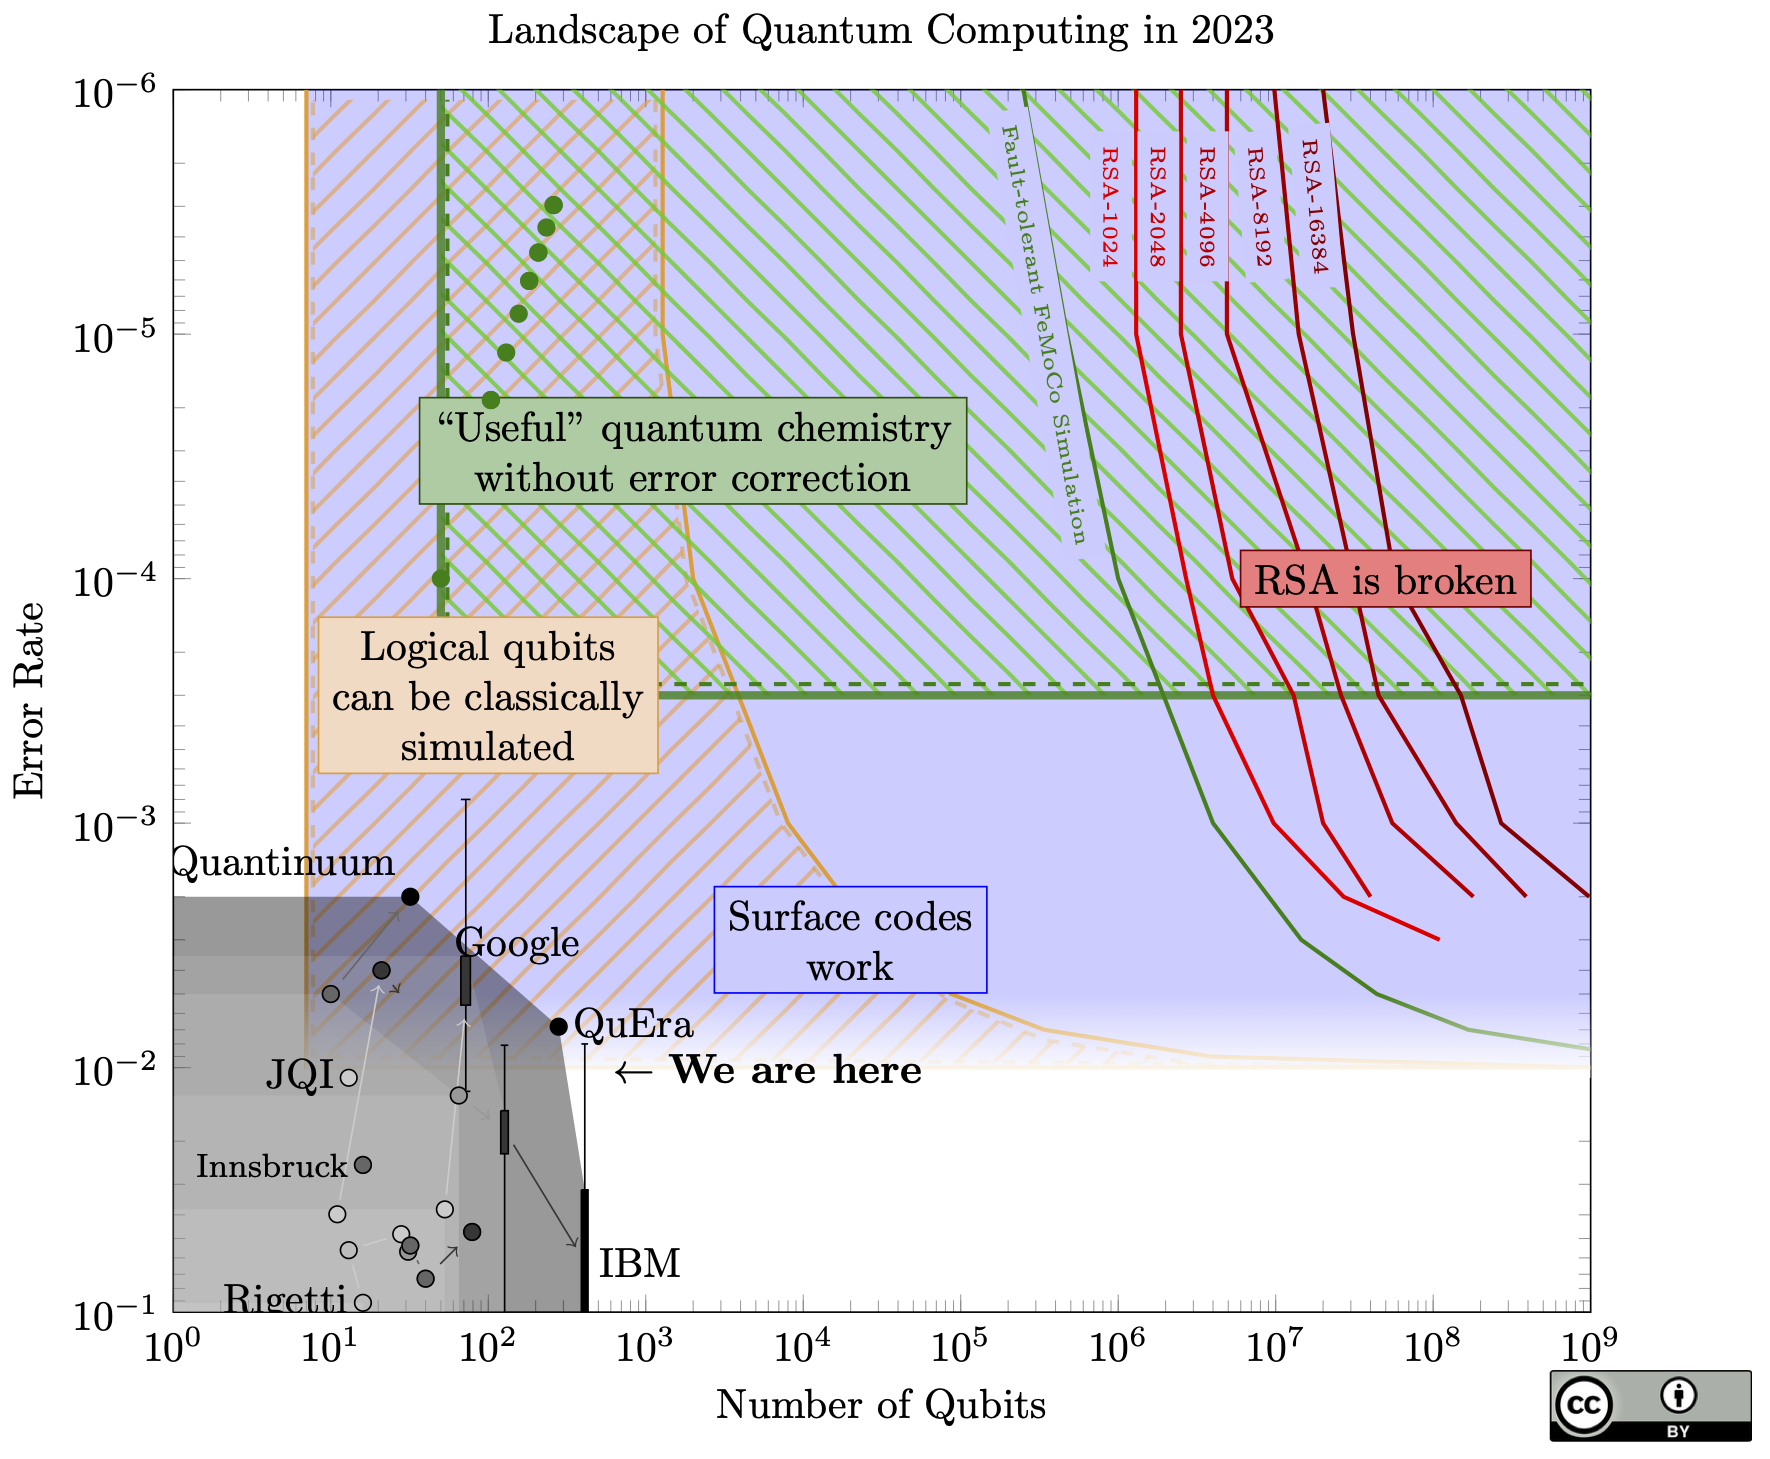
\includegraphics[scale=0.15]{figures/quantum-diagram-2023-new.png}
     \caption{\scriptsize\url{https://sam-jaques.appspot.com/quantum\_landscape}}
   \end{figure}
 \end{frame}
 
 \begin{frame}{Where are we? }
   \vspace{-3em}
   \begin{figure}
     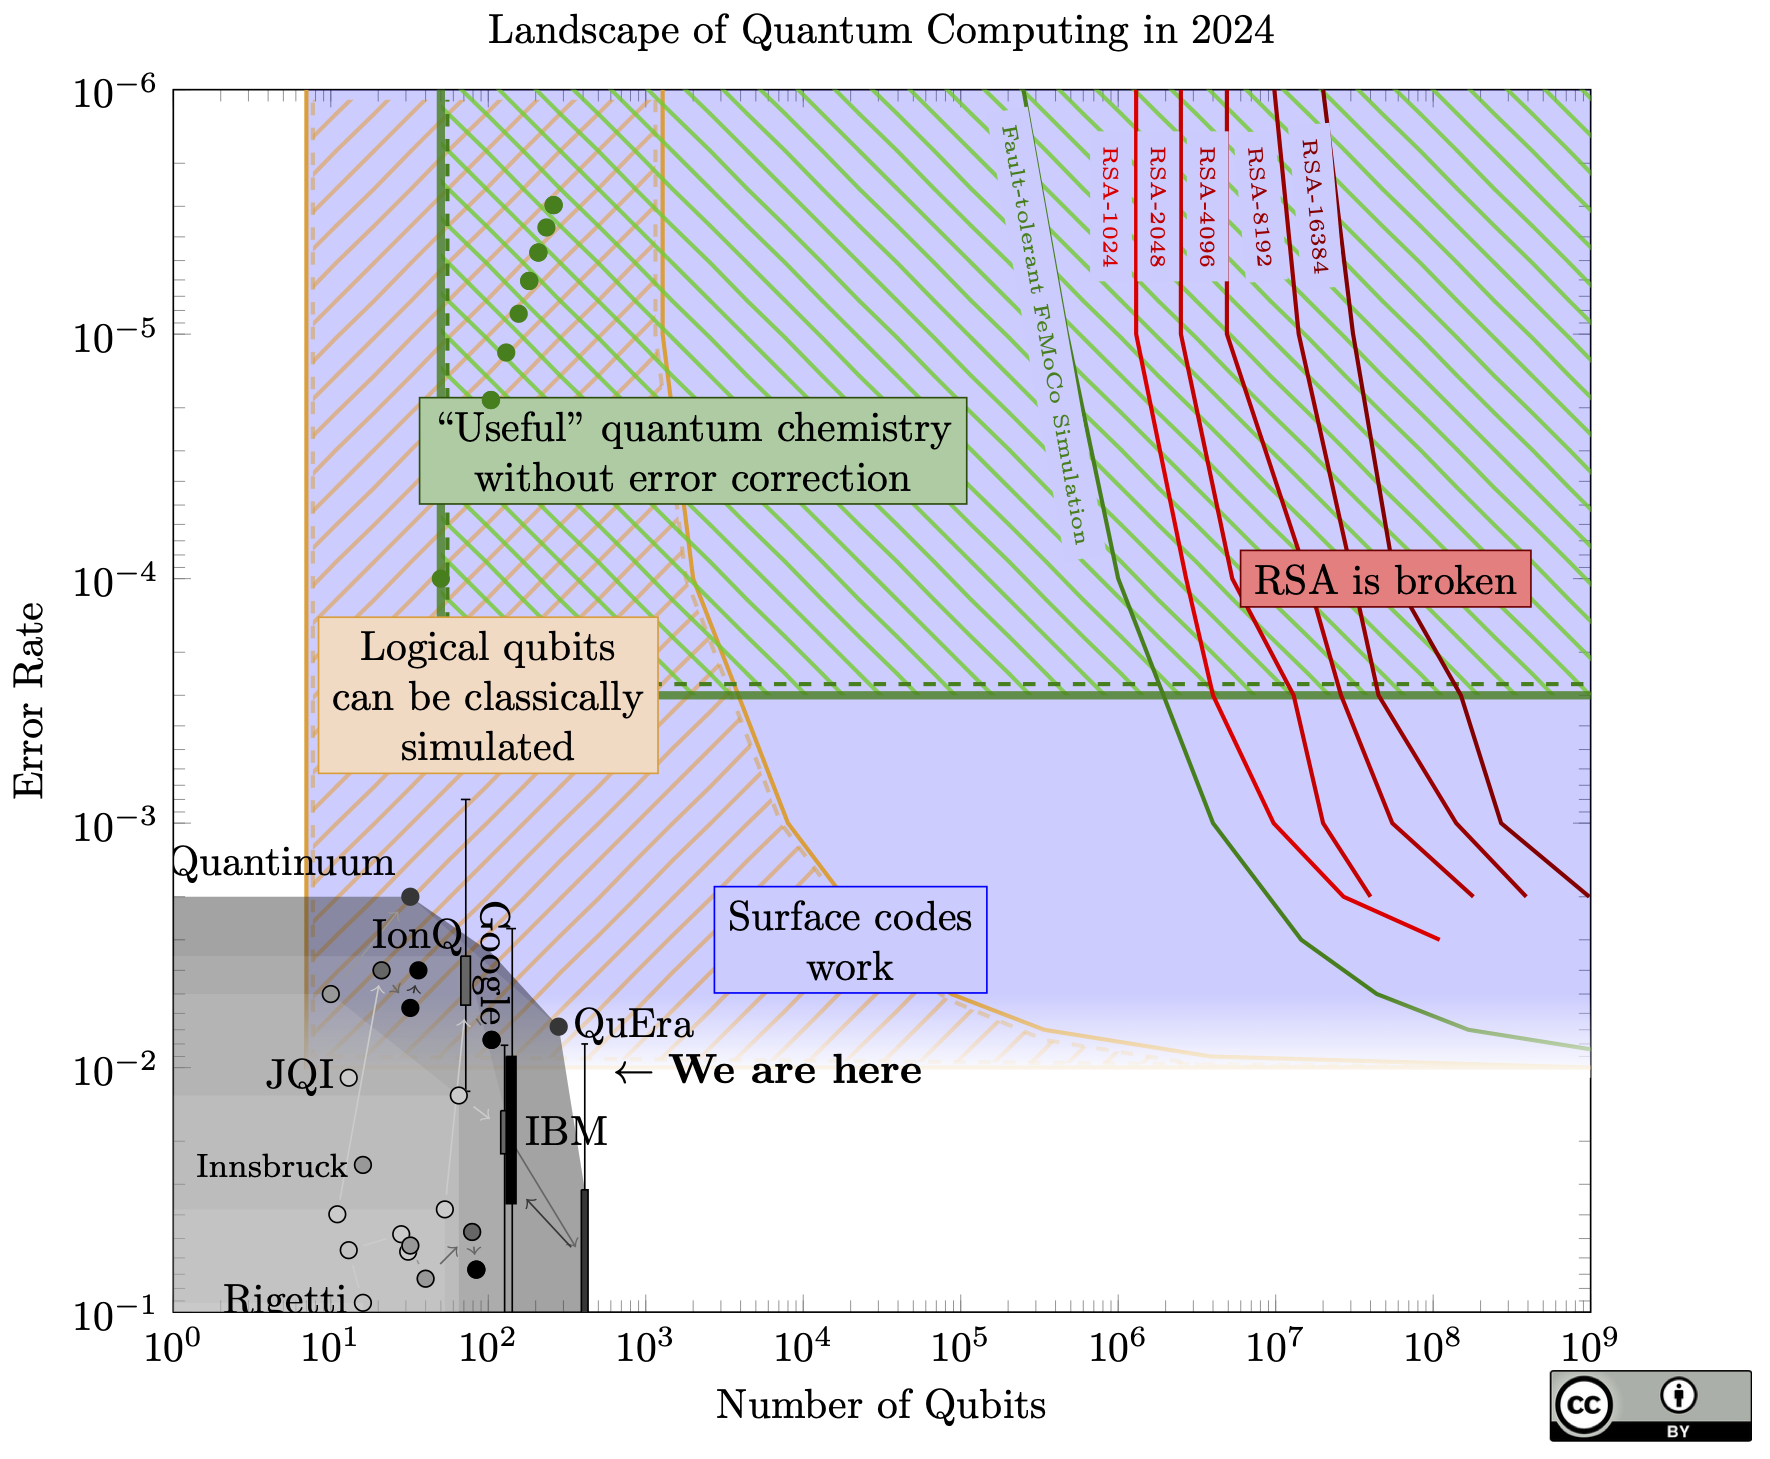
\includegraphics[scale=0.15]{figures/quantum-diagram-2024-new.png}
     \caption{\scriptsize\url{https://sam-jaques.appspot.com/quantum\_landscape}}
   \end{figure}
 \end{frame}
 
 \begin{frame}{Where are we? }
   \vspace{-3em}
   \begin{figure}
     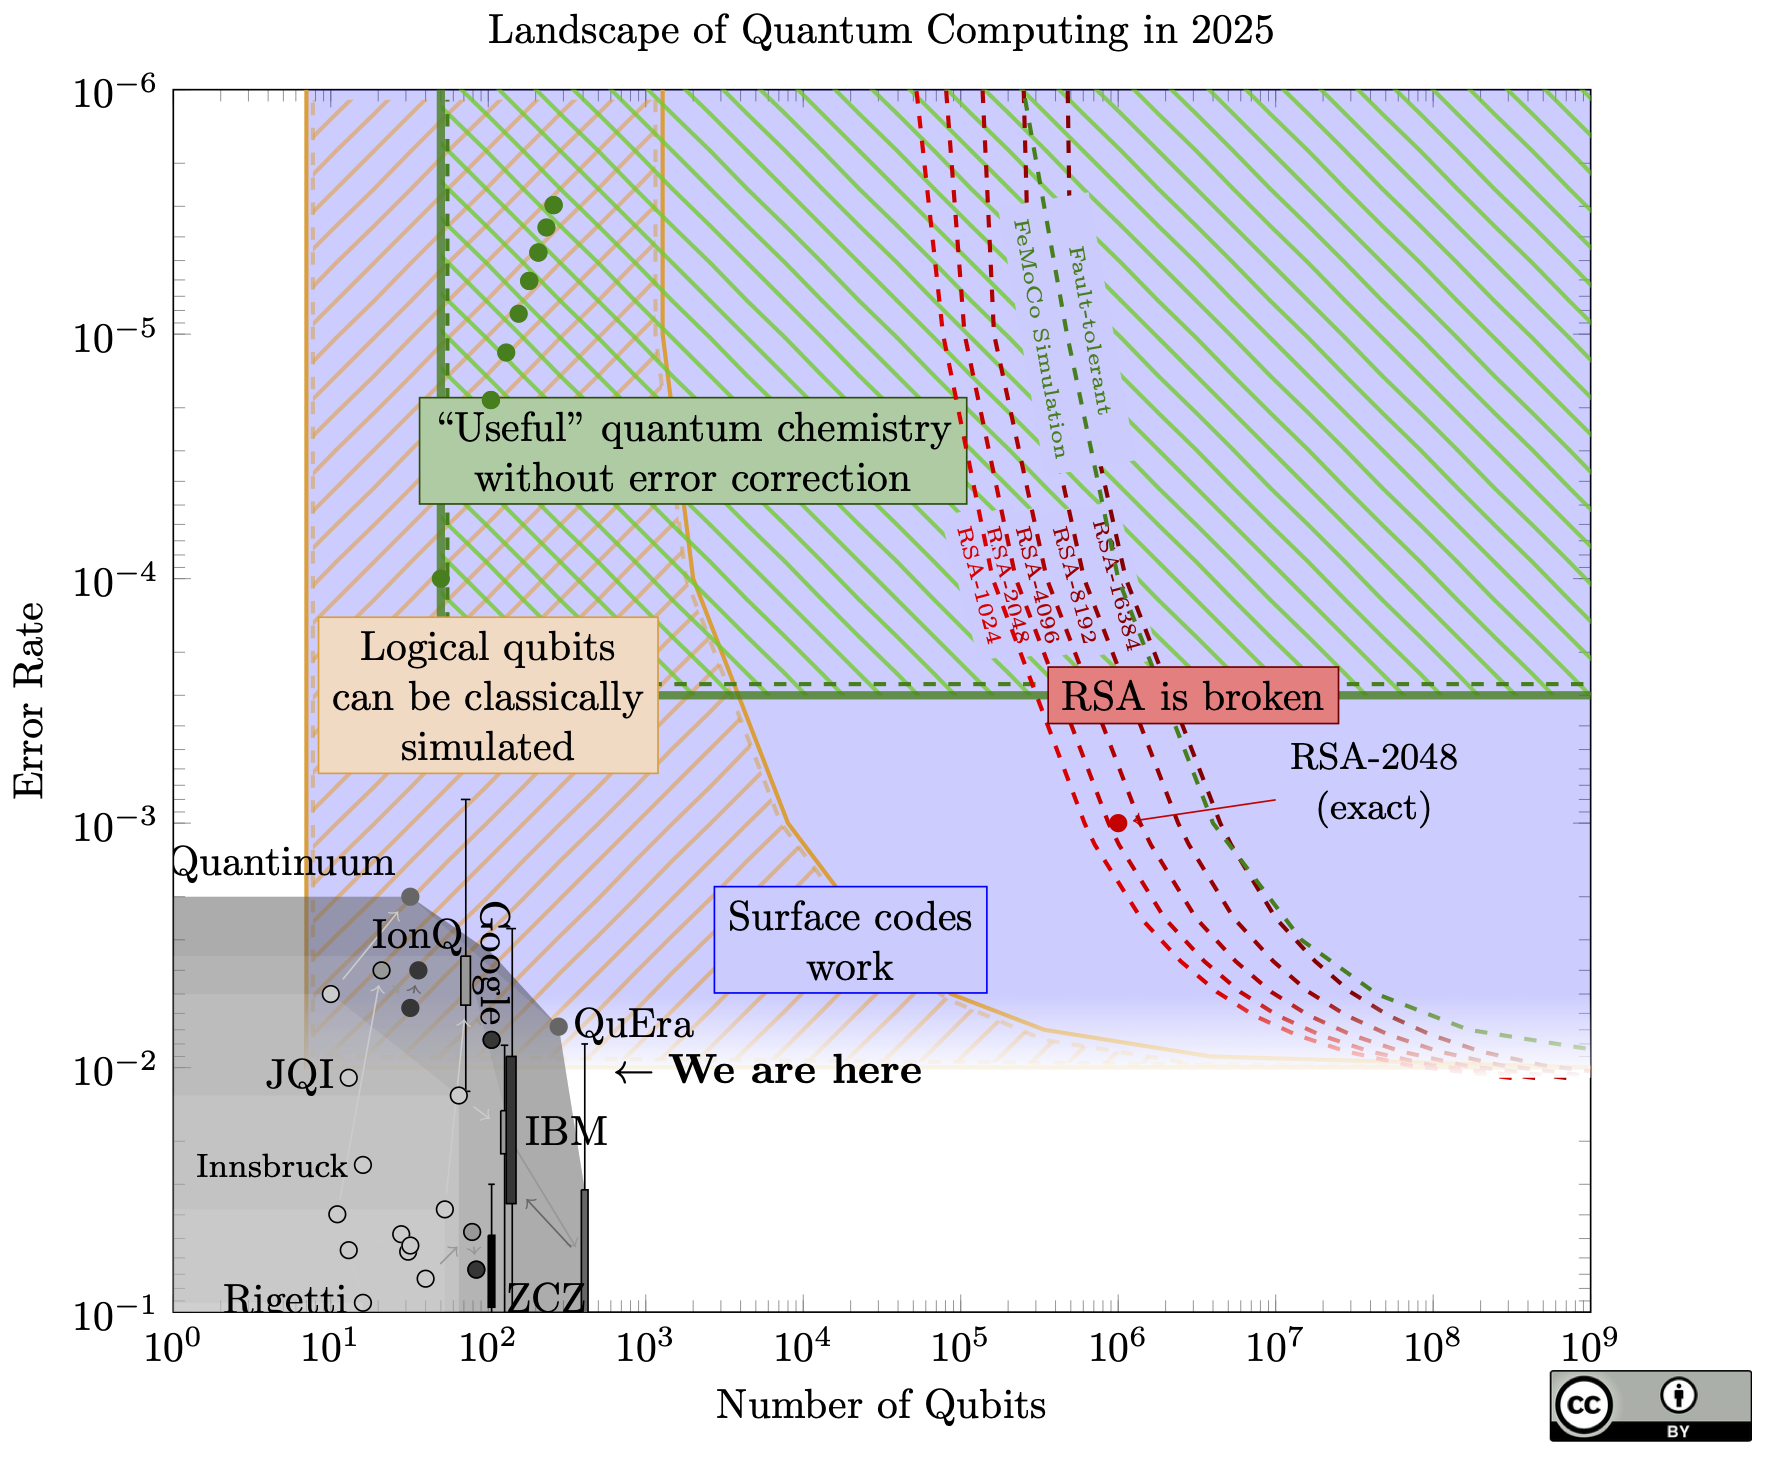
\includegraphics[scale=0.15]{figures/quantum-diagram-2025.png}
     \caption{\scriptsize\url{https://sam-jaques.appspot.com/quantum\_landscape}}
   \end{figure}
 \end{frame}
 
 \begin{frame}{Where are we? }
   \vspace{-3em}
   \begin{figure}
     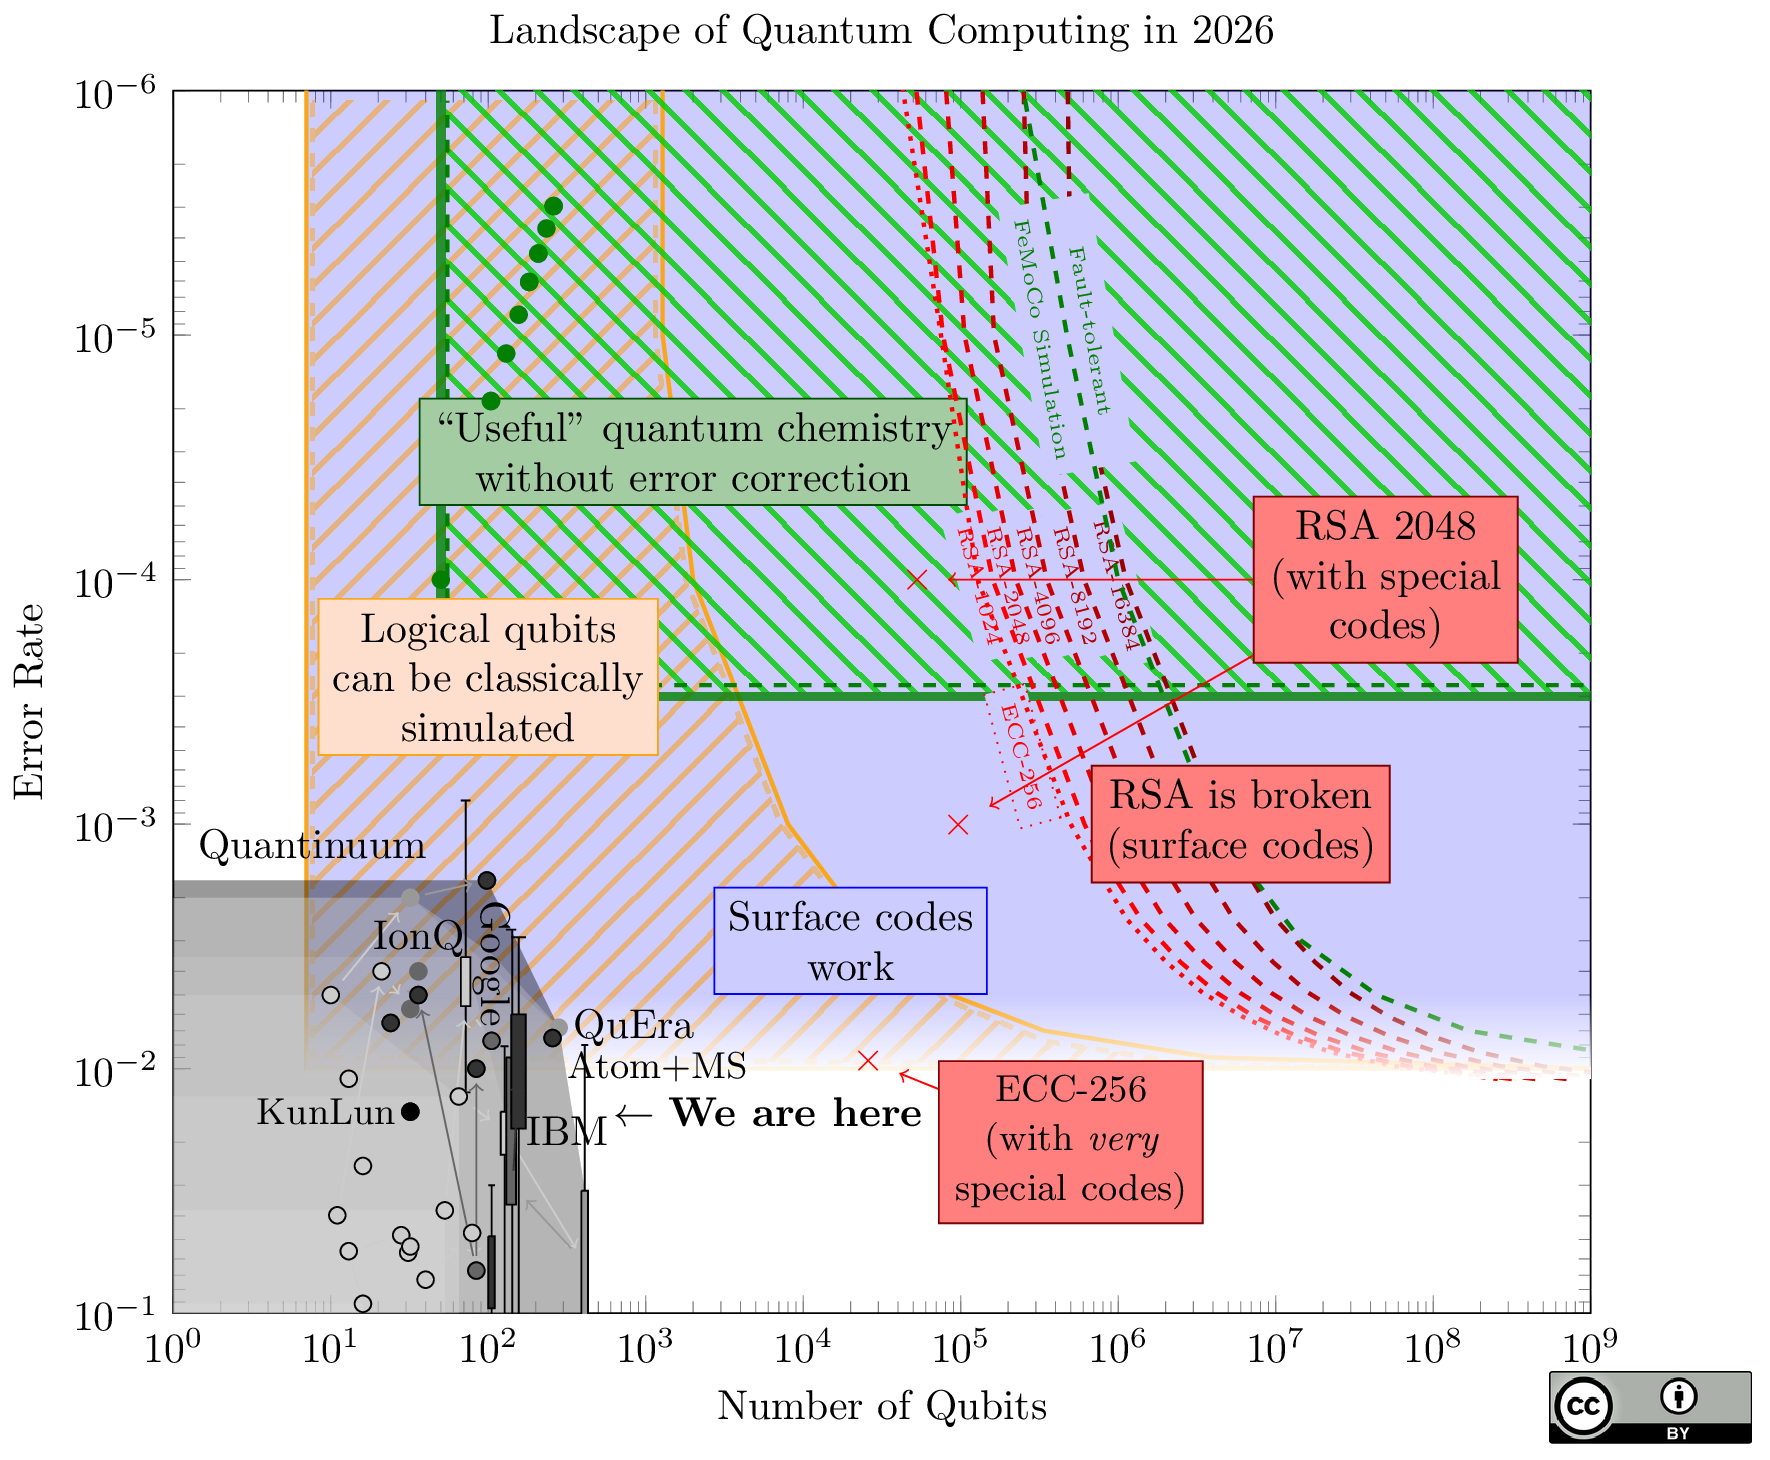
\includegraphics[scale=0.15]{figures/quantum-diagram-2026.png}
     \caption{\scriptsize\url{https://sam-jaques.appspot.com/quantum\_landscape}}
   \end{figure}
 \end{frame}


\begin{frame}{When is a scheme secure? }
  \centering
  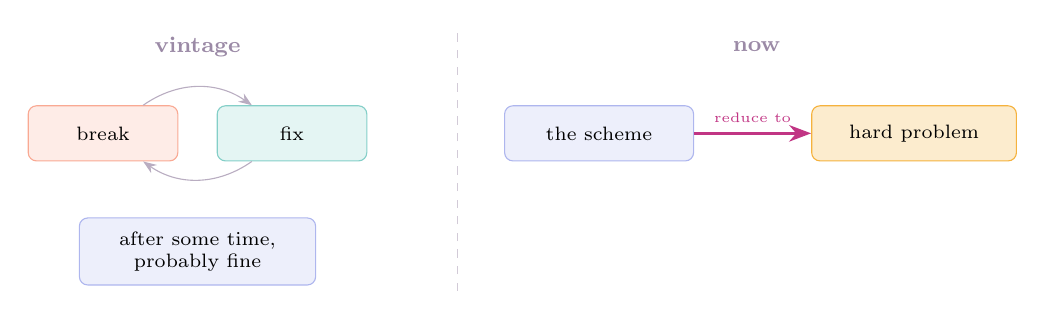
\begin{tikzpicture}[font=\scriptsize,x=1cm,y=1cm,
      b/.style={rounded corners=3pt,inner sep=5pt,align=center,
                line width=0.4pt,minimum width=19mm,minimum height=7mm}]
    \node[grey,font=\footnotesize\bfseries] at (2.1,2.6) {vintage};
    \node[b,fill=bad!12,draw=bad!55]  (br) at (0.9,1.5) {break};
    \node[b,fill=good!12,draw=good!55](fx) at (3.3,1.5) {fix};
    \draw[-{Stealth},grey!70] (br) to[bend left=35] (fx);
    \draw[-{Stealth},grey!70] (fx) to[bend left=35] (br);
    \uncover<2->{
    \node[b,fill=peri!12,draw=peri!55,minimum width=30mm] (conf) at (2.1,0)
      {after some time,\\ probably fine};
  }
    \uncover<4->{

    \draw[grey!45,dashed] (5.4,-0.5) -- (5.4,2.8);

    \node[grey,font=\footnotesize\bfseries] at (9.2,2.6) {now};
    \node[b,fill=peri!12,draw=peri!55,minimum width=24mm] (sch) at (7.2,1.5)
      {the scheme};
    \node[b,fill=warm!25,draw=warm,minimum width=26mm] (hard) at (11.2,1.5)
      {hard problem};
    \draw[-{Stealth},acc,line width=1.1pt] (sch) -- (hard)
      node[midway,above,acc,font=\tiny]{reduce to};
  }
  \end{tikzpicture}
  \vspace{1mm}
  \begin{itemize}
    \item<3-> When has enough time passed? 
    \item<4-> Reductionist security: \\ show breaking the scheme is as hard as breaking  underlying assumption
    \item<5-> Reason about model, tightness of reduction, which problem. 
  \end{itemize}
\end{frame}

\begin{frame}{Security Levels}
  \centering\footnotesize
  \begin{tabular}{c l}
    \toprule
    \textbf{NIST level}  & \textbf{at least as hard as}  \\
    \midrule
    1 & recovering an AES-128 key  \\
    2 & finding a SHA-256 collision  \\
    3 & recovering an AES-192 key  \\
    4 & finding a SHA-384 collision  \\
    5 & recovering an AES-256 key  \\
    \bottomrule
  \end{tabular}
  \vspace{2mm}
  \begin{itemize}
    \item<2-> ``$k$-bit security'' means roughly $2^{k}$ operations: 
      128 bits is AES-128,
      RSA-3072 and P-256.
    \item<3-> Rough estimate, independent of hardware, memory, target... 
    \item<4-> \alert{Quantum cost models move:} the qubit count for RSA-2048 reduced by a factor of
      twenty \\ \pause
      \cgrey{How to factor 2048 bit RSA integers with less than a million noisy qubits, Craig Gidney, \url{https://arxiv.org/pdf/2505.15917}}
  \end{itemize}
\end{frame}


% \begin{frame}{Security is an exponent, not a number}
%   \centering
%   \begin{tabular}{@{}l l l@{}}
%     \toprule
%     \textbf{problem, $n$ bits} & \textbf{best known cost} & \textbf{doubling $n$} \\
%     \midrule
%     ECDLP, generic & $2^{n/2}$ \hfill \cgood{exponential}
%       & \cgood{squares the cost} \\[2pt]
%     AES key search & $2^{n}$ \hfill \cgood{exponential}
%       & \cgood{squares the cost} \\[2pt]
%     AES, Grover & $2^{n/2}$ \hfill \cgood{exponential}
%       & \cgood{squares the cost} \\[2pt]
%     factoring, NFS & $\exp\!\bigl(1.92\, n^{1/3}(\log n)^{2/3}\bigr)$
%       \hfill \cwarm{sub-exponential} & \cwarm{$\times\,2^{40}$ or so} \\[2pt]
%     factoring, Shor & $O(n^{3})$ \hfill \cbad{polynomial}
%       & \cbad{$\times\, 8$} \\
%     \bottomrule
%   \end{tabular}
%   \vspace{3mm}
%   \begin{itemize}\footnotesize
%     \item<2-> The only thing that matters is where $n$ sits. In the
%       exponent, your key length buys security linearly. In the base,
%       it buys you a constant factor.
%     \item<3-> A 128-bit security level means $2^{128}$ operations,
%       whatever the problem. Key length is the input, not the answer:
%       256-bit ECC and 3072-bit RSA are the same claim.
%     \item<4-> \alert{Shor moves factoring and discrete log out of the
%       exponent.} Everything else on this slide stays where it was.
%   \end{itemize}
% \end{frame}


\begin{frame}{Just double the parameters}
  \centering
  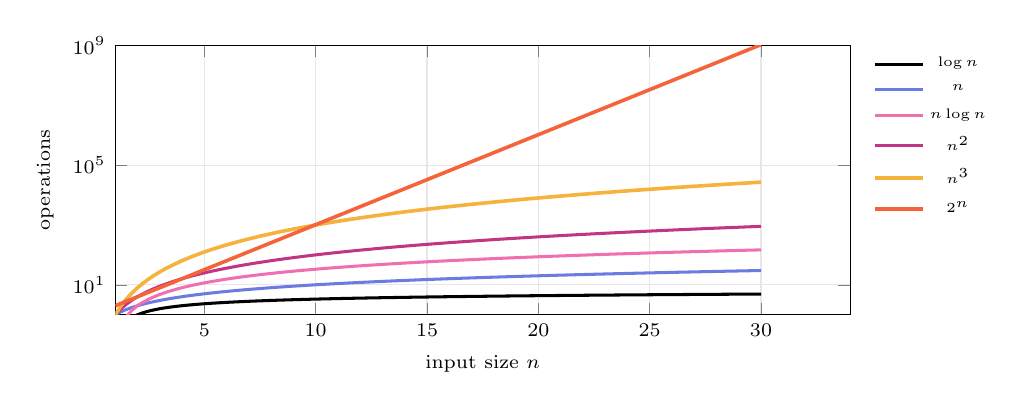
\begin{tikzpicture}[font=\scriptsize]
    \begin{axis}[
        width=0.9\textwidth,height=5.0cm,
        xlabel={input size $n$}, ylabel={operations},
        ymode=log, log basis y=10,
        domain=1:30, samples=120,
        xmin=1,xmax=34, ymin=1, ymax=1e9,
        grid=major, grid style={grey!22},
        legend style={draw=none,fill=none,at={(1.02,1.0)},
                      anchor=north west,font=\tiny,row sep=1pt},
        clip=true]
      \addplot[good,line width=1.1pt] {log2(x)};      \addlegendentry{$\log n$}
      \addplot[peri,line width=1.1pt] {x};            \addlegendentry{$n$}
      \addplot[rose,line width=1.1pt] {x*log2(x)};    \addlegendentry{$n\log n$}
      \addplot[acc,line width=1.1pt]  {x^2};          \addlegendentry{$n^{2}$}
      \addplot[warm,line width=1.3pt] {x^3};          \addlegendentry{$n^{3}$}
      \addplot[bad,line width=1.3pt]  {2^x};          \addlegendentry{$2^{n}$}
    \end{axis}
  \end{tikzpicture}
  Also doubles the work you need to do! \pause \\
  Terabytes of RSA keys

\end{frame}


\begin{frame}{About me}
  \begin{itemize}
    \item PhD Student in *:-* Privacy in a post-quantum  world *-* \pause
    \item PQ protocols, primitives and assumptions \pause
    \item deeply optimistic \pause 
  \end{itemize}
  \centering
  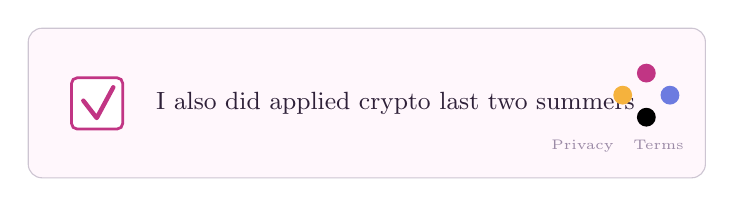
\begin{tikzpicture}[x=1cm,y=1cm,font=\small]
    \fill[blush,rounded corners=5pt,draw=grey!50,line width=0.4pt]
      (0,0) rectangle (8.6,1.9);
    \draw[acc,line width=1pt,rounded corners=2pt,fill=white]
      (0.55,0.62) rectangle (1.2,1.27);
    \draw[acc,line width=1.6pt,line cap=round,line join=round]
      (0.7,0.98) -- (0.87,0.76) -- (1.08,1.15);
    \node[anchor=west,text=ink] at (1.5,0.95) {I also did applied crypto last two summers};
    \fill[acc]  (7.85,1.33) circle (3.4pt);
    \fill[peri] (8.15,1.05) circle (3.4pt);
    \fill[good] (7.85,0.77) circle (3.4pt);
    \fill[warm] (7.55,1.05) circle (3.4pt);
    \node[anchor=east,text=grey,font=\tiny] at (8.45,0.40) {Privacy \ \ Terms};
  \end{tikzpicture} \pause \\ 

  Talk touches a lot of points. If you ever zone out, just zone back in later. 
\end{frame}

% ---------------------------------------------------------------------
\begin{frame}{When to switch to PQ? }
  \centering
  \begin{description}
    \item[\cgood{\textbf{Shared secrets are fine.}}] AES, SHA-2, HMAC:
      Grover's algorithm. \\ \pause
    \item[\cbad{\textbf{Asymmetric is vulnerable.}}] RSA,
      Diffie-Hellman, ECDSA: Shor's Algorithm.
  \end{description}
  \vspace{2em}

   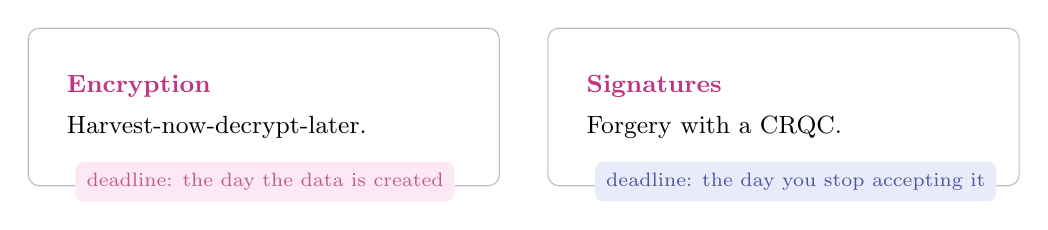
\begin{tikzpicture}[font=\small,x=1cm,y=1cm,
     card/.style={rounded corners=4pt,anchor=north west,inner sep=14pt,
       align=left,text width=5cm,minimum height=2cm,
     draw=mauve!60,fill=white,line width=0.4pt},
     tag/.style={rounded corners=3pt,anchor=north west,inner sep=4pt,
     font=\scriptsize}]
 
     \uncover<3->{
       \node[card] (enc) at (0,-1.8)
         {\cacc{\textbf{Encryption}}\\[4pt]
         Harvest-now-decrypt-later.};
     }
     \uncover<4->{
       \node[card] (sig) at (6.6,-1.8)
         {\cacc{\textbf{Signatures}}\\[4pt]
         Forgery with a CRQC.};
     }
 
      \uncover<3->{
          \node[tag,fill=rose!15,text=rose!80!black] at (0.6,-3.5)
            {deadline: the day the data is created};
        }
       \uncover<4->{
           \node[tag,fill=peri!15,text=peri!70!black] at (7.2,-3.5)
             {deadline: the day you stop accepting it};
         }
       \end{tikzpicture}
    \end{frame}
    % =====================================================================

    \heroframe{\node[chef,female,hero,shirt=black, details=pink!70!white,hat=black,hair=pink] {};}
    {the Novice}{Why does a quantum computer break cryptography?}

    % ---------------------------------------------------------------------
    \begin{frame}{A hard problem becomes easy with a \st{friend} secret}
  \centering
  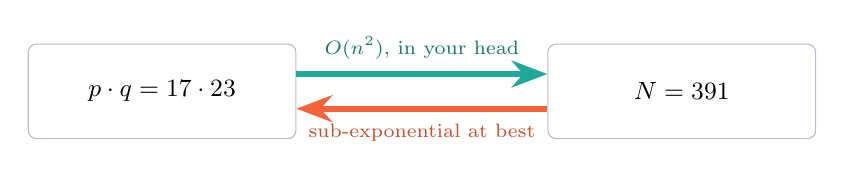
\begin{tikzpicture}[font=\small,
      b/.style={draw=mauve!60,rounded corners=3pt,fill=white,
                minimum height=12mm,minimum width=34mm,line width=0.4pt}]
    \node[b] (a) at (0,0) {$p \cdot q = 17 \cdot 23$};
    \node[b] (c) at (6.6,0) {$N = 391$};
    \draw[-{Stealth},teal,line width=2.2pt]
      ($(a.east)+(0,0.22)$) -- ($(c.west)+(0,0.22)$)
      node[midway,above=1pt,font=\scriptsize,text=teal!70!black]
      {$O(n^{2})$, in your head};
    \uncover<2->{
    \draw[-{Stealth},coral,line width=2.2pt]
      ($(c.west)+(0,-0.22)$) -- ($(a.east)+(0,-0.22)$)
      node[midway,below=1pt,font=\scriptsize,text=coral!80!black]
      {sub-exponential at best};
  }
  \end{tikzpicture}
  \vfill
  \begin{itemize}
    \item<1-> Polynomial complexity for multiplication. 
    \item<2->  general number field sieve runs in
      $\exp(O((\log N)^{1/3}(\log\log N)^{2/3}))$.
    \item<3-> NP-hard: fast verification algorithm, hard to search
    \\bounds the
      \emph{worst} instance, cryptography needs the \emph{average} instance to be hard.
    % \item<5-> RSA-4098 instantiates this with two 2048-bit primes.
    %   Public key: $N$. Private key: $p$ and $q$.
  \end{itemize}
\end{frame}

        % ---------------------------------------------------------------------
\begin{frame}{Shor reduces factoring to \emph{frequency finding}}
          \centering
          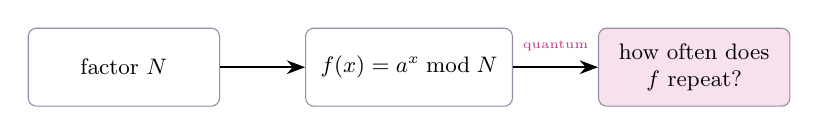
\begin{tikzpicture}[font=\small,node distance=12mm,scale=0.9,
            transform shape,
            b/.style={draw=grey,rounded corners=3pt,fill=white,align=center,
            inner sep=6pt,minimum height=11mm,minimum width=27mm}]
            \node[b] (n) {factor $N$};
            \uncover<2->{
              \node[b,right=of n] (f) {$f(x) = a^{x} \bmod N$};
            \draw[-{Stealth},thick] (n) -- (f);
            }
            \uncover<3->{
            \node[b,right=of f,fill=acc!15] (r) {how often does\\ $f$ repeat?};
            %\node[b,right=of r,fill=good!15] (fac) {$\gcd(a^{r/2}\pm 1,\,N)$};
            \draw[-{Stealth},thick] (f) -- node[above=1mm,font=\tiny,acc]{quantum} (r);
          }

            % \draw[-{Stealth},thick] (r) -- node[above=1mm,font=\tiny,grey]{algebra} (fac);
          \end{tikzpicture}

          \footnotesize\cgrey{P. Shor, 1994/1997.}

          \centering
          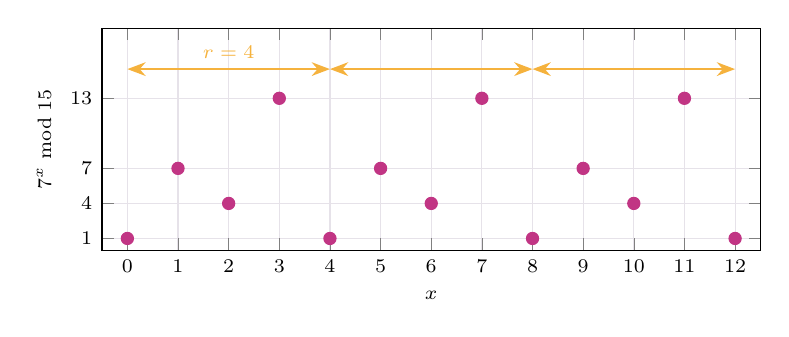
\begin{tikzpicture}[font=\scriptsize]
            \begin{axis}[
              width=0.82\textwidth,height=4.4cm,
              xlabel={$x$}, ylabel={$7^{x} \bmod 15$},
              xmin=-0.5,xmax=12.5,ymin=0,ymax=19,
              xtick={0,...,12}, ytick={1,4,7,13},
              grid=major, grid style={grey!25},
              only marks, mark size=2.2pt]
              \addplot[mark=*,acc] coordinates {
                (0,1)(1,7)(2,4)(3,13)(4,1)(5,7)(6,4)(7,13)(8,1)(9,7)(10,4)(11,13)(12,1)};
              \draw[warm,thick,{Stealth}-{Stealth}] (axis cs:0,15.5) -- (axis cs:4,15.5)
                node[midway,above=0pt,warm]{$r=4$};
              \draw[warm,thick,{Stealth}-{Stealth}] (axis cs:4,15.5) -- (axis cs:8,15.5);
              \draw[warm,thick,{Stealth}-{Stealth}] (axis cs:8,15.5) -- (axis cs:12,15.5);
            \end{axis}
          \end{tikzpicture}
          \vfill
          RSA security depends on the attacker not knowing the order of the group. 
        %   \begin{itemize}
        %     \item $\langle 7 \rangle = \{1,7,4,13\}
        %       \le \mathbb{Z}_{15}^{*}$, $x \mapsto 7^x$ is a homomorphism from $\mathbb{Z}$ onto a
        %       \alert{cyclic group},  period $r$ is the order of that group.
        %     \item $\gcd(7^{2}-1,15)=3$, $\gcd(7^{2}+1,15)=5$ 
         %   \end{itemize}
        \end{frame}
% 
%         \begin{frame}{What the QFT does to one basis state}
%   \centering
%   \[
%     \mathrm{QFT}:\quad \lvert x\rangle \;\longmapsto\;
%     \frac{1}{\sqrt{2^{t}}}\sum_{c=0}^{2^{t}-1} \omega^{xc}\,\lvert c\rangle,
%     \qquad \omega = e^{2\pi i/2^{t}}
%   \]
%   \begin{tikzpicture}[font=\scriptsize,x=1cm,y=1cm]
%     \foreach \c [evaluate=\c as \ang using {\c*40}] in {0,...,7}{
%       \draw[grey!35] ({\c*1.35},0) circle (0.42);
%       \draw[-{Stealth},peri,thick] ({\c*1.35},0) -- ++({\ang}:0.42);
%       \node[below=6pt,grey] at ({\c*1.35},-0.42) {$c=\c$};}
%     \node[anchor=west,align=left,text width=2.2cm] at (9.9,0)
%       {one amplitude per $c$, all the same size, only the
%        \cacc{phase} turns};
%   \end{tikzpicture}
%   \vspace{1mm}
%   \begin{itemize}\small
%     \item<1-> It is a change of basis, nothing more: position basis
%       out, frequency basis in. Unitary, so no information is created.
%     \item<2-> A single $x$ spreads over every $c$ with a phase that
%       winds at rate $x$. Measuring here would be useless.
%     \item<3-> The point is what happens when we feed it a
%       \emph{superposition}: the phase ramps of the terms either line
%       up or they do not.
%   \end{itemize}
% \end{frame}
% 
% \begin{frame}{Why only the right frequencies survive}
%   \centering
%   \[
%     \frac{1}{\sqrt{M}}\sum_{j=0}^{M-1}\lvert x_{0}+jr\rangle
%     \;\longmapsto\;
%     \underbrace{\omega^{x_{0}c}}_{\text{global phase}}
%     \cdot \frac{1}{\sqrt{M\,2^{t}}}
%     \underbrace{\sum_{j=0}^{M-1}\omega^{jrc}}_{\text{geometric sum}}
%     \;\lvert c\rangle
%   \]
%   \begin{tikzpicture}[font=\scriptsize,x=1cm,y=1cm,scale=0.85,transform shape]
%     \draw[grey!35] (0,0) circle (1.0);
%     \foreach \k in {0,...,5}{
%       \draw[-{Stealth},peri] (0,0) -- ({12+\k*3}:0.95);}
%     \draw[-{Stealth},good,line width=1.4pt] (0,0) -- (20:1.0);
%     \node[below=1.15cm,align=center,good] at (0,0)
%       {$rc/2^{t}$ near an integer\\ \cgrey{phases agree, sum is large}};
%     \draw[grey!35] (4.6,0) circle (1.0);
%     \foreach \k in {0,...,5}{
%       \draw[-{Stealth},peri] (4.6,0) -- ++({\k*60+10}:0.95);}
%     \fill[bad] (4.6,0) circle (2.2pt);
%     \node[below=1.15cm,align=center,bad] at (4.6,0)
%       {anything else\\ \cgrey{phases spread, sum is zero}};
%     \node[anchor=west,align=left,text width=4.4cm] at (6.2,0.1)
%       {$\bigl|\sum_j \omega^{jrc}\bigr| =
%        \left|\dfrac{\sin(\pi M r c/2^{t})}{\sin(\pi r c/2^{t})}\right|$};
%   \end{tikzpicture}
%   \vspace{-1mm}
%   \begin{itemize}\small
%     \item<1-> $x_{0}$ leaves as a phase of modulus one, so it cannot
%       touch a probability: only the spacing is visible.
%     \item<2-> The $M$ arrows all step by $2\pi rc/2^{t}$. Whole turns
%       stack, anything else closes a polygon, so the peaks sit at
%       $c \approx k\,2^{t}/r$.
%   \end{itemize}
% \end{frame}
% 
% 
%         \begin{frame}{Fourier sampling: reading the spacing as a frequency}
%   \centering
%   \begin{tikzpicture}[font=\scriptsize]
%     \begin{axis}[
%         name=left,width=0.45\textwidth,height=3.5cm,
%         ybar,bar width=2.4pt,
%         xlabel={$x$ in the first register},
%         ymin=0,ymax=1.25,xmin=-1,xmax=16,
%         ytick=\empty,xtick={1,5,9,13},
%         grid=none,axis y line*=left,axis x line*=bottom]
%       \addplot[fill=peri,draw=peri] coordinates {(1,1)(5,1)(9,1)(13,1)};
%     \end{axis}
%     \begin{axis}[
%         name=right,at={($(left.east)+(1.6cm,0)$)},anchor=west,
%         width=0.45\textwidth,height=3.5cm,
%         ybar,bar width=2.4pt,
%         xlabel={measured $c$},
%         ymin=0,ymax=1.25,xmin=-1,xmax=16,
%         ytick=\empty,xtick={0,4,8,12},
%         grid=none,axis y line*=left,axis x line*=bottom]
%       \addplot[fill=acc,draw=acc] coordinates {(0,1)(4,1)(8,1)(12,1)};
%     \end{axis}
%     \draw[-{Stealth},thick,warm] ($(left.east)+(0.2cm,0.2cm)$)
%       -- node[above,font=\tiny,warm]{$\mathrm{QFT}^{\dagger}$}
%       ($(right.west)+(-0.2cm,0.2cm)$);
%   \end{tikzpicture}
%   \vfill
%   \begin{itemize}
%     \item<1-> After the measurement the first register is a comb:
%       every $x \equiv x_{0} \pmod r$, nothing else. The offset
%       $x_{0}$ is random and useless.
%     \item<2-> The transform is blind to that offset and sees only the
%       spacing. Amplitudes cancel everywhere except at multiples of
%       $2^{t}/r$.
%     \item<3-> One run gives one $c \approx k\,2^{t}/r$ for a random
%       $k$. Continued fractions of $c/2^{t}$ give $k/r$ in lowest
%       terms, so a couple of runs pin down $r$.
%     \item<4-> This is interference, not parallelism: the wrong answers
%       are made to cancel.
%   \end{itemize}
% \end{frame}
% 
% \begin{frame}{Shor reduces factoring to \emph{frequency finding}}
%   \centering
%   \begin{tikzpicture}[font=\small,node distance=12mm,scale=0.9,transform shape,
%       b/.style={draw=grey!60,rounded corners=3pt,fill=white,align=center,
%                 inner sep=6pt,minimum height=11mm,minimum width=27mm,
%                 line width=0.4pt}]
%     \node[b] (n) {factor $N$};
%     \node[b,right=of n] (f) {$f(x) = a^{x} \bmod N$};
%     \node[b,right=of f,fill=acc!12] (r) {the period $r$\\ of $f$};
%     \node[b,right=of r,fill=good!15] (fac) {$\gcd(a^{r/2}\pm 1,\,N)$};
%     \uncover<2->{\draw[-{Stealth},thick,grey] (n) -- (f);}
%     \uncover<3->{\draw[-{Stealth},thick,acc] (f)
%       -- node[above=1mm,font=\tiny,acc]{quantum} (r);}
%     \uncover<4->{\draw[-{Stealth},thick,grey] (r)
%       -- node[above=1mm,font=\tiny,grey]{Euclid} (fac);}
%   \end{tikzpicture}
%   \vfill
%   \begin{itemize}
%     \item<2-> Pick any $a$ coprime to $N$. Factoring is now a question
%       about one function.
%     \item<3-> The only quantum step: find how often that function
%       repeats. Polynomial in $\log N$.
%     \item<4-> Everything after it is classical arithmetic.
%   \end{itemize}
%   \vfill
%   \footnotesize\cgrey{P. Shor, 1994/1997.}
% \end{frame}

 %\begin{frame}{Why a period gives you a factor}
 %  \centering
 %  \begin{tikzpicture}[font=\small,node distance=6mm,
 %      b/.style={draw=grey!60,rounded corners=3pt,fill=white,align=center,
 %                inner sep=7pt,minimum height=10mm,line width=0.4pt}]
 %    \node[b] (p1) {$a^{r} \equiv 1 \pmod N$};
 %    \node[b,right=8mm of p1,fill=acc!10] (p2)
 %      {$\bigl(a^{r/2}\bigr)^{2} \equiv 1 \pmod N$};
 %    \node[b,right=8mm of p2,fill=warm!20] (p3)
 %      {$\bigl(a^{r/2}-1\bigr)\bigl(a^{r/2}+1\bigr) \equiv 0 \pmod N$};
 %    \draw[-{Stealth},thick,grey] (p1) -- (p2);
 %    \draw[-{Stealth},thick,grey] (p2) -- (p3);
 %  \end{tikzpicture}
 %  \vfill
 %  \begin{itemize}
 %    \item<1-> $N$ divides the product but neither factor, so each
 %      factor shares a real divisor with $N$. One $\gcd$ finds it.
 %    \item<2-> $a=7$, $N=15$, $r=4$: $7^{2}=49\equiv 4$, and
 %      $4^{2}\equiv 1$. So $4$ is a square root of $1$ that is neither
 %      $1$ nor $-1$.
 %    \item<3-> $\gcd(4-1,15)=3$ and $\gcd(4+1,15)=5$.
 %    \item<4-> Fails if $r$ is odd or $a^{r/2}\equiv -1$. Draw a new
 %      $a$: success probability per attempt is at least $1/2$.
 %  \end{itemize}
 %\end{frame}
 %
 %\begin{frame}{What repeats, and why}
 %  \centering
 %  \begin{tikzpicture}[font=\scriptsize]
 %    \begin{axis}[
 %        width=0.82\textwidth,height=4.4cm,
 %        xlabel={$x$}, ylabel={$7^{x} \bmod 15$},
 %        xmin=-0.5,xmax=12.5,ymin=0,ymax=19,
 %        xtick={0,...,12}, ytick={1,4,7,13},
 %        grid=major, grid style={grey!25},
 %        only marks, mark size=2.2pt]
 %      \addplot[mark=*,acc] coordinates {
 %        (0,1)(1,7)(2,4)(3,13)(4,1)(5,7)(6,4)(7,13)(8,1)(9,7)(10,4)(11,13)(12,1)};
 %      \draw[warm,thick,{Stealth}-{Stealth}] (axis cs:0,15.5) -- (axis cs:4,15.5)
 %        node[midway,above=0pt,warm]{$r=4$};
 %      \draw[warm,thick,{Stealth}-{Stealth}] (axis cs:4,15.5) -- (axis cs:8,15.5);
 %      \draw[warm,thick,{Stealth}-{Stealth}] (axis cs:8,15.5) -- (axis cs:12,15.5);
 %    \end{axis}
 %  \end{tikzpicture}
 %  \vfill
 %  \begin{itemize}
 %    \item<1-> $\langle 7\rangle = \{1,7,4,13\} \le \mathbb{Z}_{15}^{*}$,
 %      and $x \mapsto 7^{x}$ is a homomorphism from $\mathbb{Z}$ onto it.
 %    \item<2-> The period is the \alert{order of the group}, so period
 %      finding is order finding, and the kernel of that homomorphism is
 %      $r\mathbb{Z}$.
 %    \item<3-> Same statement for discrete logarithms, elliptic curves,
 %      and any commutative group action. One subroutine, four dead
 %      assumptions.
 %  \end{itemize}
 %\end{frame}
 %
 %
 %\begin{frame}{The circuit}
 %  \centering
 %  \begin{tikzpicture}[font=\scriptsize,x=1cm,y=1cm,
 %      g/.style={draw=grey!70,fill=white,rounded corners=2pt,
 %                minimum height=7mm,minimum width=7mm,line width=0.4pt}]
 %    \draw[grey!70] (0,1.2) -- (10.4,1.2);
 %    \draw[grey!70] (0,0) -- (7.6,0);
 %    \node[anchor=east] at (-0.1,1.2) {$\lvert 0\rangle^{\otimes t}$};
 %    \node[anchor=east] at (-0.1,0) {$\lvert 1\rangle$};
 %    \node[g,fill=acc!12] at (1.1,1.2) {$H$};
 %    \node[g,fill=warm!25,minimum width=30mm,minimum height=9mm] (u) at (4.2,0)
 %      {$\lvert y\rangle \mapsto \lvert a^{x}y \bmod N\rangle$};
 %    \fill[acc] (4.2,1.2) circle (2.2pt);
 %    \draw[acc,thick] (4.2,1.2) -- (u.north);
 %    \node[g,fill=acc!12,minimum width=16mm] at (6.6,1.2) {$\mathrm{QFT}^{\dagger}$};
 %    \node[g] at (8.8,1.2) {measure};
 %    \node[anchor=west,align=left,text width=2.4cm,grey] at (9.6,0.2)
 %      {second register\\ is discarded};
 %    \node[anchor=north,grey] at (1.1,0.7) {equal superposition of all $x$};
 %  \end{tikzpicture}
 %  \vfill
 %  \begin{itemize}
 %    \item<1-> One modular exponentiation, evaluated on every $x$ at
 %      once. This is the whole cost, in qubits and in depth.
 %    \item<2-> Measuring the second register collapses the first onto
 %      the $x$ sharing that value: an arithmetic progression of step
 %      $r$.
 %    \item<3-> $\mathrm{QFT}^{\dagger}$ turns spacing into frequency.
 %      The measurement returns a multiple of $2^{t}/r$, and continued
 %      fractions recover $r$.
 %  \end{itemize}
 %\end{frame}

        \begin{frame}{Blinding operations}
  \centering
  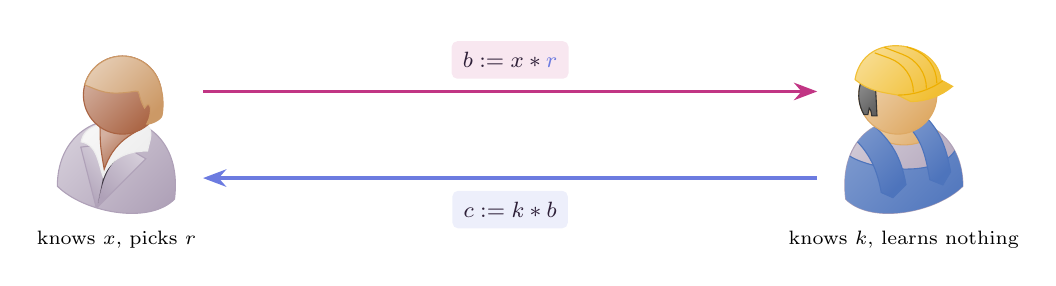
\begin{tikzpicture}[font=\small,x=1cm,y=1cm,
      env/.style={rounded corners=2pt,inner sep=4pt,font=\footnotesize}]
    \node[alice,minimum size=1.5cm,shirt=mauve,hair=brown,mirrored] (c) at (0,0) {};
    \node[builder,minimum size=1.5cm,shirt=mauve] (s) at (10,0) {};
    \node[font=\scriptsize,below=1mm of c] {knows $x$, picks $r$};
    \node[font=\scriptsize,below=1mm of s] {knows $k$, learns nothing};

    \uncover<2->{
      \draw[-{Stealth},acc,line width=1.2pt] (1.1,0.55) -- (8.9,0.55);
      \node[env,fill=acc!12,text=ink] at (5,0.95)
        {$b := x * \textcolor{peri}{r}$};}

    \uncover<3->{
      \draw[-{Stealth},peri,line width=1.2pt] (8.9,-0.55) -- (1.1,-0.55);
      \node[env,fill=peri!12,text=ink] at (5,-0.95) {$c := k * b$};}
      

  \end{tikzpicture}
  \vspace{2mm}
\end{frame}

        % ---------------------------------------------------------------------
        \begin{frame}{Hidden shifts in commutative settings: Kuperberg}
          \centering
          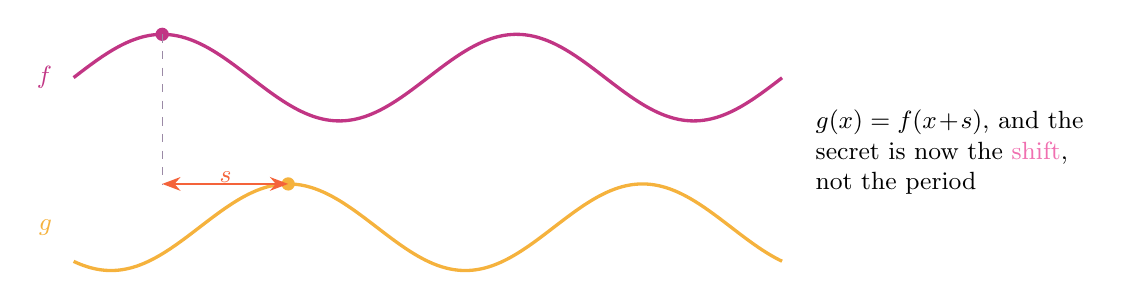
\begin{tikzpicture}[font=\small]
            \draw[acc,very thick,smooth,samples=200,domain=0:9]
              plot (\x,{0.55*sin(\x*80)});
            \draw[warm,very thick,smooth,samples=200,domain=0:9]
              plot (\x,{0.55*sin((\x-1.6)*80)-1.9});
            \node[left,acc] at (-0.15,0) {$f$};
            \node[left,warm] at (-0.15,-1.9) {$g$};
            \fill[acc] (1.125,0.55) circle (2.4pt);
            \fill[warm] (2.725,-1.35) circle (2.4pt);
            \draw[grey,dashed] (1.125,0.55) -- (1.125,-1.35);
            \draw[bad,thick,{Stealth}-{Stealth}] (1.125,-1.35) -- (2.725,-1.35);
            \node[bad,above] at (1.93,-1.45) {$s$};
            \node[right,align=left,text width=3.4cm] at (9.3,-0.95)
              {$g(x) = f(x+s)$, and the secret is now the \cbad{shift}, not the period};
          \end{tikzpicture}
          \vfill
          \begin{itemize}
            \item Same commutative structure, secret moved from \emph{period} to \emph{offset}.
            \item Then quantum computers have \alert{subexponential} advantage.
          \end{itemize}
          \vfill
          \footnotesize\cgrey{G. Kuperberg. A subexponential-time quantum
            algorithm for the dihedral hidden subgroup problem. SIAM J.\
          Comput.\ 35(1), 2005.}
        \end{frame}

        % ---------------------------------------------------------------------
        \begin{frame}[standout]
          Remove the frequency.
        \end{frame}

        % =====================================================================

        \heroframe{
          \node[bride, veil=black, shirt=pink,hero,shirt=rose,hair=pink] (e) {};
          % a beer
          \begin{scope}[shift={(2.5,-1.5)},scale=1.5]
            \fill[warm!35,draw=warm!70,thick,rounded corners=1pt] (0,0) rectangle (0.8,1.25);
            \fill[white,draw=warm!70,thick,rounded corners=2pt] (-0.05,1.18) rectangle (0.85,1.52);
            \draw[warm!70,thick] (0.8,0.35) .. controls (1.3,0.45) and (1.3,0.95) .. (0.8,1.05);
        \end{scope}}
        {the Enjoyer}{What Alice did last night.}


        \newcommand{\lat}{%
  \foreach \y in {-2,0,2,4}{\foreach \x in {-3,...,14}{
    \pgfmathparse{int(mod(\x-\y,3))}
    \ifnum\pgfmathresult=0 \fill[peri!55] (\x,\y) circle (1.9pt);\fi}}}

\begin{frame}{The same lattice, described twice}
  \centering
  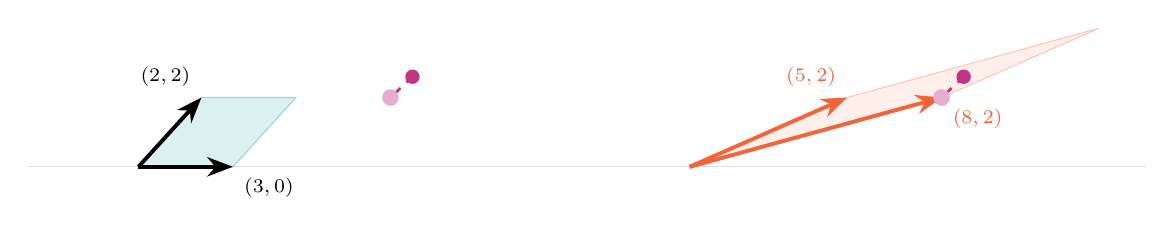
\begin{tikzpicture}[x=0.40cm,y=0.44cm,font=\scriptsize,>={Stealth}]
    \begin{scope}
      \lat
      \draw[grey!30] (-3.5,0) -- (14.5,0);
      \fill[good!16,draw=good!45] (0,0) -- (3,0) -- (5,2) -- (2,2) -- cycle;
      \draw[good,line width=1.4pt,->] (0,0) -- (3,0) node[below right]{$(3,0)$};
      \draw[good,line width=1.4pt,->] (0,0) -- (2,2) node[above left]{$(2,2)$};
      \uncover<3->{
        \fill[acc] (8.7,2.6) circle (2.6pt);
        \draw[acc,line width=1pt,dashed] (8.7,2.6) -- (8,2);
        \fill[acc!40] (8,2) circle (3pt);}
    \end{scope}
    \begin{scope}[shift={(17.5,0)}]
      \uncover<2->{
        \lat
        \draw[grey!30] (-3.5,0) -- (14.5,0);
        \fill[bad!10,draw=bad!35] (0,0) -- (8,2) -- (13,4) -- (5,2) -- cycle;
        \draw[bad,line width=1.4pt,->] (0,0) -- (8,2) node[below right]{$(8,2)$};
        \draw[bad,line width=1.4pt,->] (0,0) -- (5,2) node[above left]{$(5,2)$};}
      \uncover<3->{
        \fill[acc] (8.7,2.6) circle (2.6pt);
        \draw[acc,line width=1pt,dashed] (8.7,2.6) -- (8,2);
        \fill[acc!40] (8,2) circle (3pt);}
    \end{scope}
  \end{tikzpicture}
\end{frame}

\begin{frame}{All about that base}
  \centering
  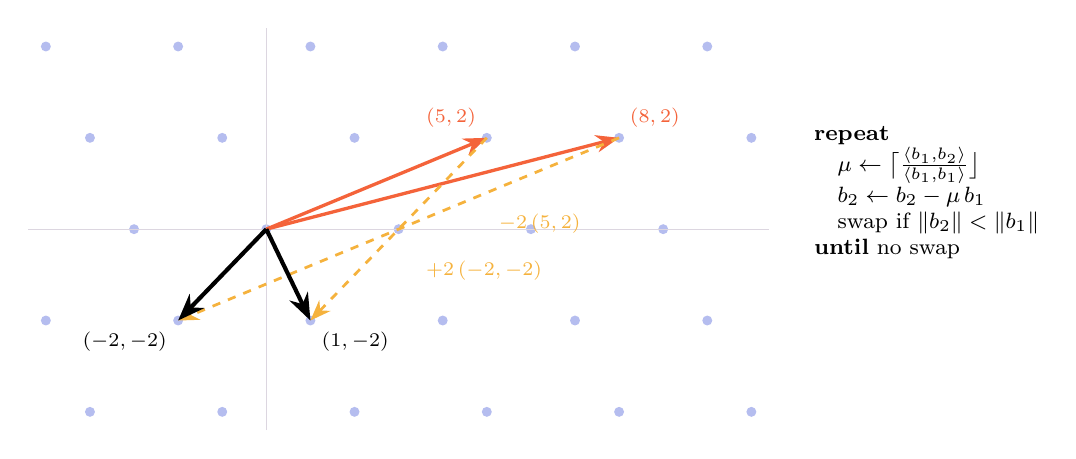
\begin{tikzpicture}[x=0.56cm,y=0.58cm,font=\scriptsize,>={Stealth}]
    \foreach \y in {-4,-2,0,2,4}{\foreach \x in {-5,...,11}{
      \pgfmathparse{int(mod(\x-\y,3))}
      \ifnum\pgfmathresult=0 \fill[peri!50] (\x,\y) circle (1.8pt);\fi}}
    \draw[grey!35] (-5.4,0) -- (11.4,0);
    \draw[grey!35] (0,-4.4) -- (0,4.4);
    \draw[->,bad,line width=1.2pt] (0,0) -- (8,2) node[above right]{$(8,2)$};
    \draw[->,bad,line width=1.2pt] (0,0) -- (5,2) node[above left]{$(5,2)$};
    \uncover<2->{
      \draw[->,warm,line width=1pt,dashed] (8,2) -- (-2,-2);
      \node[warm,anchor=north,font=\scriptsize] at (6.2,0.55) {$-2\,(5,2)$};}
    \uncover<3->{
      \draw[->,warm,line width=1pt,dashed] (5,2) -- (1,-2);
      \node[warm,anchor=west,font=\scriptsize] at (3.4,-0.9) {$+2\,(-2,-2)$};}
    \uncover<4->{
      \draw[->,good,line width=1.5pt] (0,0) -- (-2,-2) node[below left]{$(-2,-2)$};
      \draw[->,good,line width=1.5pt] (0,0) -- (1,-2) node[below right]{$(1,-2)$};}
    \node[anchor=west,align=left,font=\footnotesize] at (12.2,0.8)
      {\textbf{repeat}\\
       \quad $\mu \leftarrow \bigl\lceil \tfrac{\langle b_1,b_2\rangle}
         {\langle b_1,b_1\rangle} \bigr\rfloor$\\
       \quad $b_2 \leftarrow b_2 - \mu\, b_1$\\
       \quad swap if $\lVert b_2\rVert < \lVert b_1\rVert$\\
       \textbf{until} no swap};
  \end{tikzpicture}
  \vspace{1mm}
  \begin{itemize}\small
    \item<5-> Subtract the nearest multiple, swap, repeat. Replace the
      inner products with division and this is Euclid's algorithm.
    \item<6-> LLL is the approximate version.
  \end{itemize}
\end{frame}
% ---------------------------------------------------------------------
%         \begin{frame}{Approximate values: where did Alice lose her earrings? }
%           TODO map of Telep
%           Alice lost her earrings somewhere between 
%           %Шумска and Хероја Пинкија
% 
%           , she reconstructed her walk, but her friend has a good map to know roughly where to look. 
%         \end{frame}
%         \begin{frame}{Approximate values: where did Alice lose her earrings? }
%           \centering
%           \[
%             \mathbf{A}\,\mathbf{s} \;+\; \mathbf{e} \;=\; \mathbf{b}
%             \qquad\text{with \cacc{$\mathbf{e}$ small}}
%           \]
%           \begin{tikzpicture}[font=\scriptsize,scale=0.8]
%             \foreach \i in {0,...,6}{\foreach \j in {0,...,3}{
%             \fill[acc!70] ({\i*1.35+\j*0.46},{\j*1.15}) circle (2.1pt);}}
%               \draw[acc!25] (0,0) -- (1.35,0) -- (1.81,1.15) -- (0.46,1.15) -- cycle;
%               \fill[bad] (5.0,2.65) circle (2.6pt) node[right,bad]{\ $\mathbf{b}$};
%               \fill[good] (4.44,2.30) circle (2.6pt) node[below,good]{$\mathbf{A}\mathbf{s}$};
%               \draw[good,very thick,-{Stealth}] (4.44,2.30) -- (4.94,2.61);
%             \end{tikzpicture}
%             \vfill
%             \begin{itemize}
%               \item Without the small error: Gaussian elimination
%               \item With it: find the nearest grid point to a point that is
%                 slightly off the grid. Nobody knows how, quantum or not.
%               \item Ships as ML-KEM, ML-DSA, Falcon.
%             \end{itemize}
%           \end{frame}
% 

\begin{frame}{Lattices: linear algebra with some noise}
  \centering
  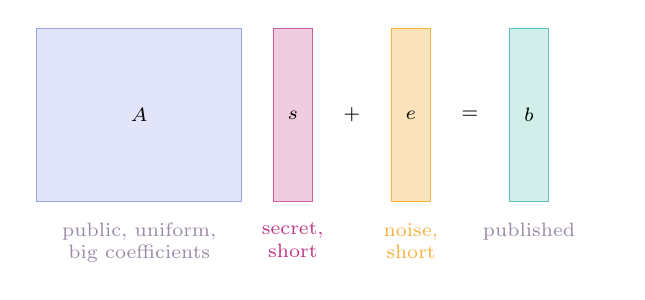
\begin{tikzpicture}[font=\scriptsize,x=1cm,y=1cm]
    \fill[peri!20,draw=peri!70] (0,0) rectangle (2.6,2.2);
    \node at (1.3,1.1) {$A$};
    \node[grey,anchor=north,align=center,text width=2.6cm] at (1.3,-0.15)
      {public, uniform,\\ big coefficients};
    \fill[acc!25,draw=acc!80] (3.0,0) rectangle (3.5,2.2);
    \node at (3.25,1.1) {$s$};
    \node[acc,anchor=north,align=center,text width=2.0cm] at (3.25,-0.15)
      {secret,\\ short};
    \node at (4.0,1.1) {$+$};
    \fill[warm!35,draw=warm] (4.5,0) rectangle (5.0,2.2);
    \node at (4.75,1.1) {$e$};
    \node[warm,anchor=north,align=center,text width=2.0cm] at (4.75,-0.15)
      {noise,\\ short};
    \node at (5.5,1.1) {$=$};
    \fill[good!20,draw=good!70] (6.0,0) rectangle (6.5,2.2);
    \node at (6.25,1.1) {$b$};
    \node[grey,anchor=north,align=center,text width=2.0cm] at (6.25,-0.15)
      {published};
  \end{tikzpicture}
  \vspace{4mm}
  \begin{itemize}\footnotesize
    \item<2-> Given $A$ and $b$, find $s$. \\\pause \alert{Drop $e$ and this is
      Gaussian elimination}. \pause
    \item<3-> with $e$ need lattice reduction
    \item<4-> Everything else is optimization: \pause  \\ Rings and modules to shrink the key, rounding for determinism
  \end{itemize}
\end{frame}

\begin{frame}{A well-studied problem}
  \begin{itemize}
    \item system of univariate linear equations over integers with some noise\pause 
    \item Number fields, $p$-adic numbers, Abelian varieties:... can be restated as a  lattice\\ \pause
      efficient general lattice  reduction solve far more than cryptography. \pause
    \item lattices have been studied as long as elliptic curves, but patents limited use \pause
    \item \alert{Lattice reduction started as an attack} \pause 
      broke
      knapsack cryptosystems in the 80's \pause 
  \end{itemize}
  \bigskip
  \begin{center}
    \cgrey{Rise from the ashes of cryptanalysis.}
  \end{center}
\end{frame}



\begin{frame}{Codes: the same equations, counted differently}
  \centering
  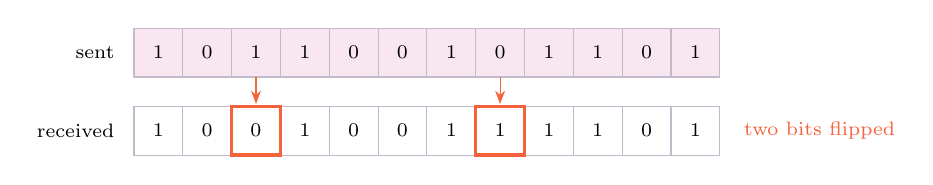
\begin{tikzpicture}[font=\scriptsize,x=0.62cm,y=0.62cm]
    \foreach \i/\v in {0/1,1/0,2/1,3/1,4/0,5/0,6/1,7/0,8/1,9/1,10/0,11/1}{
      \draw[fill=acc!12,draw=grey!60] (\i,1.9) rectangle ++(1,1);
      \node at (\i+0.5,2.4) {\v};}
    \node[anchor=east] at (-0.2,2.4) {sent};
    \foreach \i/\v in {0/1,1/0,2/0,3/1,4/0,5/0,6/1,7/1,8/1,9/1,10/0,11/1}{
      \draw[fill=white,draw=grey!60] (\i,0.3) rectangle ++(1,1);
      \node at (\i+0.5,0.8) {\v};}
    \node[anchor=east] at (-0.2,0.8) {received};
    \foreach \i in {2,7}{
      \draw[bad,line width=1.2pt] (\i,0.3) rectangle ++(1,1);
      \draw[bad,-{Stealth}] (\i+0.5,1.9) -- (\i+0.5,1.35);}
    \node[bad,anchor=west] at (12.3,0.8) {two bits flipped};
  \end{tikzpicture}
  \vspace{2em}
  \begin{itemize}
    \item<2-> Underdetermined linear system\pause \\ sparse solution instead of small
    \item<3-> Secret is efficient decoder
    \item<4-> Public: the same
      code, scrambled until it looks random.
    \item<4-> McEliece, 1978. Older than RSA is old
      \item<5-> \st{conservative choice.} Distinguisher attack
  \end{itemize}
  \note{Alice visits her grandfather: back in my day we had one tool
  for everything. Encryption, decryption, getting the TV to work, we
  built the house with it. The house in question took a lot of hits.}
\end{frame}

\begin{frame}{What a distinguisher actually means}
  \centering
  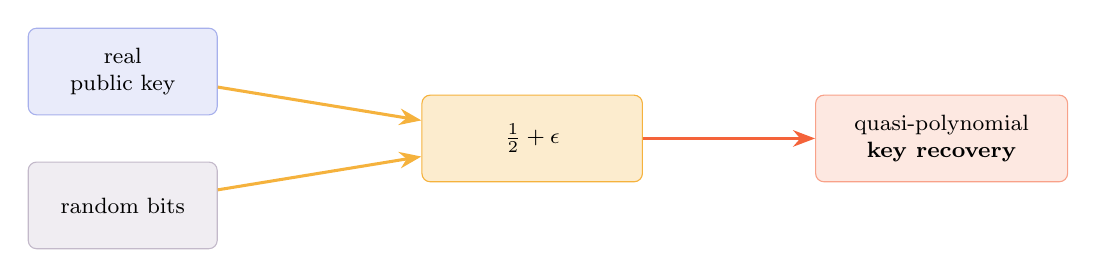
\begin{tikzpicture}[font=\footnotesize,x=1cm,y=1cm,
      b/.style={rounded corners=3pt,inner sep=6pt,minimum width=24mm,
                minimum height=11mm,align=center,line width=0.4pt}]
    \node[b,fill=peri!15,draw=peri!60] (k) at (0,0.85) {real\\ public key};
    \node[b,fill=grey!15,draw=grey!60] (r) at (0,-0.85) {random bits};
    \node[b,fill=warm!25,draw=warm,minimum width=28mm] (d) at (5.2,0)
      {$\frac{1}{2}+\epsilon$};
    \draw[-{Stealth},warm,line width=1.1pt] (k) -- (d);
    \draw[-{Stealth},warm,line width=1.1pt] (r) -- (d);
    \uncover<3->{
      \node[b,fill=bad!15,draw=bad!60,minimum width=32mm] (a) at (10.4,0)
        {quasi-polynomial\\ \textbf{key recovery}};
      \draw[-{Stealth},bad,line width=1.1pt] (d) -- (a);}
  \end{tikzpicture}
  \vspace{3mm}
  \begin{itemize}
    \item<2-> Why care if someone can tell your
      public key from noise? 
    \item<3-> \alert{ key has previously unknown structure}
      \item<4-> structure enables cryptanalysis 
    \item<5-> distinguisher became a key
      recovery in a few weeks
    \item<4-> BIKE and HQC are untouched
  \end{itemize}
  \cgrey{\scriptsize Quasipolynomial Cryptanalysis of the McEliece Cryptosystem (or: PIR Meets McEliece) \\ Ghoshal, Ishai, Jain, Sun, \url{ia.cr/2026/1630}}
\end{frame}

%           \begin{frame}{But \$name told me lattices are broken quantumly}
% 
%             Dihedral cosets
%             also, lattices are so important in math, breaking CVP would solve so many other areas
% 
%             pretty fundamental problem
% 
%             
%           \end{frame}

% preamble: the shared icon
\newcommand{\ovicon}[1]{%
  \begin{tikzpicture}[scale=#1,baseline=(current bounding box.center)]
    \fill[peri!30,draw=peri!70] (0,0.45) rectangle (0.9,1.35);
    \fill[warm!35,draw=warm]    (0.9,0.45) rectangle (1.35,1.35);
    \fill[warm!35,draw=warm]    (0,0) rectangle (0.9,0.45);
    \fill[white,draw=bad,line width=0.7pt] (0.9,0) rectangle (1.35,0.45);
  \end{tikzpicture}}

\begin{frame}{Multivariate: hide an easy system inside a hard-looking one}
  \centering
  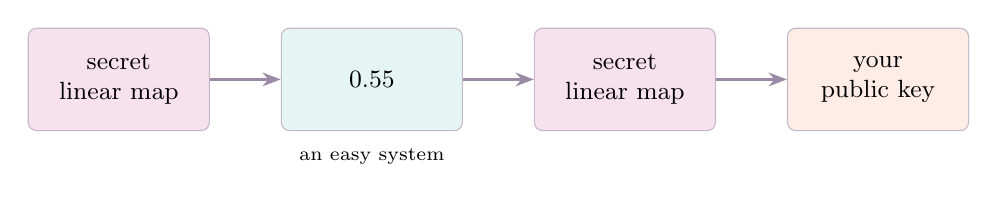
\begin{tikzpicture}[font=\small,node distance=9mm,
      b/.style={draw=grey!60,rounded corners=3pt,fill=white,minimum height=13mm,
                minimum width=23mm,align=center,line width=0.4pt}]
    \node[b,fill=acc!15] (s) {secret\\ linear map};
    \node[b,fill=good!12,right=of s] (f) {\ovicon{0.55}};
    \node[below=1mm of f,font=\scriptsize,good] {an easy system};
    \node[b,fill=acc!15,right=of f] (t) {secret\\ linear map};
    \node[b,fill=bad!12,right=of t] (p) {your\\ public key};
    \draw[-{Stealth},thick,grey] (s)--(f);
    \draw[-{Stealth},thick,grey] (f)--(t);
    \draw[-{Stealth},thick,grey] (t)--(p);
  \end{tikzpicture}
  \vspace{3mm}
  \begin{itemize}
    \item<2-> Solving random quadratic equations over a finite field
      is NP-hard, and no quantum algorithm helps.
    \item<3-> \alert{No noise anywhere.} Every equation holds exactly.
      The only thing hiding the structure is the two linear maps, so
      attacks aim straight at them.
    \item<4-> 96-byte signatures, public keys in the tens of
      kilobytes, and a habit of dying suddenly.
  \end{itemize}
 \end{frame}

\begin{frame}{The easy system: oil and vinegar}
  \centering
  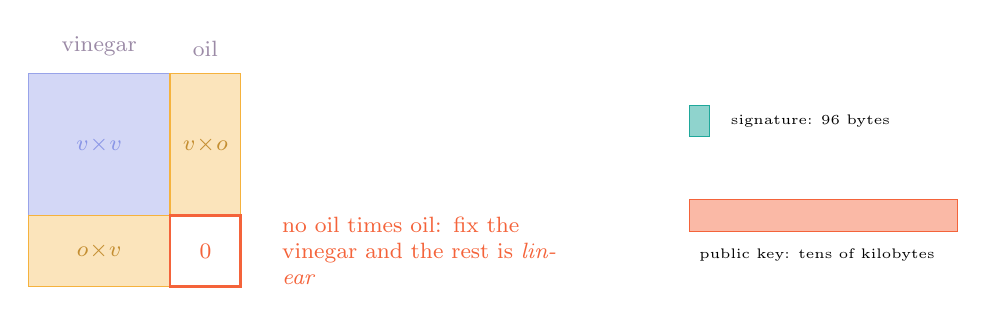
\begin{tikzpicture}[font=\footnotesize,x=1cm,y=1cm]
    \fill[peri!30,draw=peri!70] (0,0.9) rectangle (1.8,2.7);
    \fill[warm!35,draw=warm]    (1.8,0.9) rectangle (2.7,2.7);
    \fill[warm!35,draw=warm]    (0,0)   rectangle (1.8,0.9);
    \fill[white,draw=bad,line width=1pt] (1.8,0) rectangle (2.7,0.9);
    \node[bad] at (2.25,0.45) {$0$};
    \node[peri!80] at (0.9,1.8) {$v\!\times\!v$};
    \node[warm!80!black] at (2.25,1.8) {$v\!\times\!o$};
    \node[warm!80!black] at (0.9,0.45) {$o\!\times\!v$};
    \node[anchor=south,grey] at (0.9,2.8) {vinegar};
    \node[anchor=south,grey] at (2.25,2.8) {oil};
    \node[bad,anchor=west,align=left,text width=3.6cm] at (3.1,0.45)
      {no oil times oil: fix the vinegar and the rest is \emph{linear}};
    \begin{scope}[shift={(8.4,0.4)}]
      \fill[good!50,draw=good] (0,1.5) rectangle (0.25,1.9);
      \node[anchor=west,font=\tiny] at (0.4,1.7) {signature: 96 bytes};
      \fill[bad!45,draw=bad] (0,0.3) rectangle (3.4,0.7);
      \node[anchor=west,font=\tiny] at (0,0.0) {public key: tens of kilobytes};
    \end{scope}
  \end{tikzpicture}
  \vspace{2mm}
  \begin{itemize}\footnotesize
    \item<2-> Signing: guess the vinegar, solve the linear rest.
      Forging without the secret maps means finding the hidden oil
      subspace.
    \item<3-> \alert{Balanced} oil and vinegar died in 1998
      (Kipnis-Shamir). \alert{Unbalanced}, two or three times as much
      vinegar, is still standing after twenty-five years.
    \item<4-> Every attempt to shrink that public key with more
      structure has been risky. Rainbow, a layered variant, fell in a
      weekend on a laptop in 2022.
  \end{itemize}
\end{frame}



          % ---------------------------------------------------------------------
          \begin{frame}{Alice walks home alone at night}
            \centering
            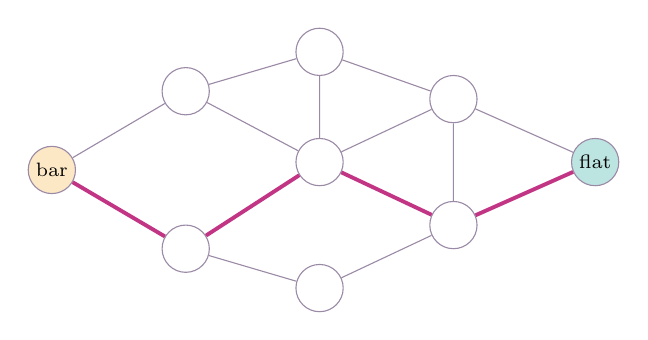
\begin{tikzpicture}[font=\scriptsize,
              v/.style={circle,draw=grey,fill=white,minimum size=6mm,inner sep=0}]
              \node[v,fill=warm!30] (s) at (0,0) {bar};
              \node[v] (b1) at (1.7,1.0) {};
              \node[v] (b2) at (1.7,-1.0) {};
              \node[v] (b3) at (3.4,1.5) {};
              \node[v] (b4) at (3.4,0.1) {};
              \node[v] (b5) at (3.4,-1.5) {};
              \node[v] (b6) at (5.1,0.9) {};
              \node[v] (b7) at (5.1,-0.7) {};
              \node[v,fill=good!30] (h) at (6.9,0.1) {flat};
              \draw[grey] (s)--(b1) (s)--(b2) (b1)--(b3) (b1)--(b4) (b2)--(b4) (b2)--(b5)
              (b3)--(b6) (b4)--(b6) (b4)--(b7) (b5)--(b7) (b6)--(h) (b7)--(h)
              (b3)--(b4) (b6)--(b7);
              \draw[acc,line width=1.4pt] (s)--(b2)--(b4)--(b7)--(h);
            \end{tikzpicture}
            \vfill
            \begin{itemize}
              \item Start: Bar, End: Got home safe text \pause
              \item \alert{Nobody can reconstruct the path.}\pause
              \item Nodes are elliptic curves, steps are maps between them\pause :
                Isogeny walk!
            \end{itemize}
          \end{frame}

          % ---------------------------------------------------------------------

          \begin{frame}{Isogenies: small, elegant, and a lot of work}
            \begin{itemize}
              \item SQIsign: 148-byte signatures \\ pause Public key and signature together fit in a
                tweet. \pause
              \item Signing is slow, \pause constant-time implementation is still
                open, \pause and the security assumption is the youngest of the lot.\pause
              \item CSIDH is vulnerable to Kuperberg \pause
              \item SIDH, the previous favourite, was broken in an afternoon in
                2022.
            \end{itemize}
          \end{frame}

          \begin{frame}[standout]
            You young people with your fancy math!  \\ We know how to build cryptogrpahy
          \end{frame}
          % ---------------------------------------------------------------------
          \begin{frame}{Symmetric: One way to signatures}
  \centering
  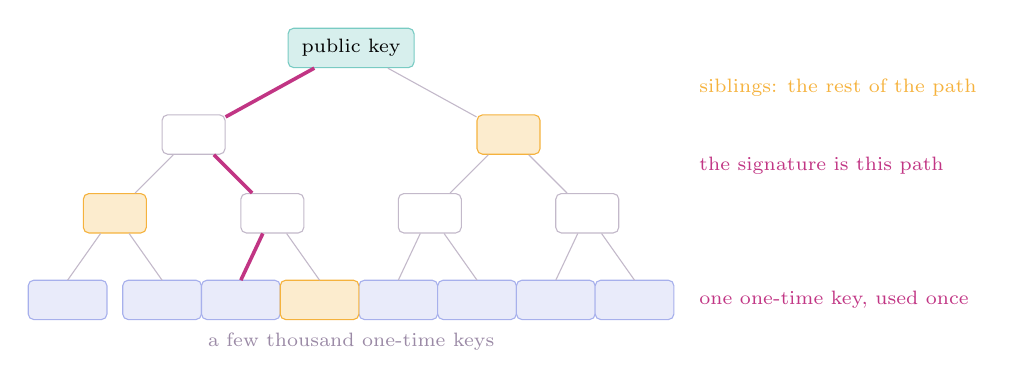
\begin{tikzpicture}[font=\scriptsize,x=1cm,y=1cm,
      n/.style={rounded corners=2pt,draw=grey!60,fill=white,
                minimum width=8mm,minimum height=5mm,line width=0.4pt},
      lf/.style={rounded corners=2pt,draw=peri!60,fill=peri!15,
                minimum width=10mm,minimum height=5mm,line width=0.4pt}]
    \node[n,fill=good!18,draw=good!60,minimum width=16mm] (root) at (4,2.4)
      {public key};
    \node[n] (l) at (2,1.3) {};
    \node[n,fill=warm!25,draw=warm] (r) at (6,1.3) {};
    \node[anchor=west,warm] at (8.3,1.9) {siblings: the rest of the path};
    \node[n,fill=warm!25,draw=warm] (a) at (1,0.3) {};
    \node[n] (b) at (3,0.3) {};
    \node[n] (c) at (5,0.3) {}; \node[n] (d) at (7,0.3) {};
    \foreach \x in {0.4,1.6,2.6,4.6,5.6,6.6,7.6}{\node[lf] at (\x,-0.8) {};}
    \node[lf,fill=warm!25,draw=warm] at (3.6,-0.8) {};
    \draw[grey!60] (root)--(l) (root)--(r) (l)--(a) (l)--(b) (r)--(c) (r)--(d);
    \foreach \x/\p in {0.4/a,1.6/a,2.6/b,3.6/b,4.6/c,5.6/c,6.6/d,7.6/d}{
      \draw[grey!60] (\x,-0.55) -- (\p);}
    \draw[acc,line width=1.3pt] (2.6,-0.55) -- (b);
    \draw[acc,line width=1.3pt] (b) -- (l) -- (root);
    \node[acc,anchor=west] at (8.3,-0.8) {one one-time key, used once};
    \node[acc,anchor=west] at (8.3,0.9) {the signature is this path};
    \node[grey,anchor=north] at (4,-1.1) {a few thousand one-time keys};
  \end{tikzpicture}
  \vspace{2mm}
  \begin{itemize}\small
    \item<2-> A hash turns a secret into a one-time key. 
    \item<3-> Clunky: either keep state and never reuse a leaf, or
       go stateless and large
    \item<4-> Security reduces to underlying hash
      function. We need one anyways, somewhere
  \end{itemize}
\end{frame}

% \begin{frame}{Signatures from nothing but a circuit}
%   \centering
%   \begin{tikzpicture}[font=\scriptsize,x=1cm,y=1cm,
%       s/.style={rounded corners=3pt,minimum width=17mm,minimum height=9mm,
%                 line width=0.4pt,align=center}]
%     \node[s,fill=peri!15,draw=peri!60] (s1) at (0,0) {share 1};
%     \node[s,fill=peri!15,draw=peri!60] (s2) at (2.1,0) {share 2};
%     \node[s,fill=peri!15,draw=peri!60] (s3) at (4.2,0) {share 3};
%     \node[s,fill=bad!12,draw=bad!60] (s4) at (6.3,0) {share 4};
%     \node[grey,anchor=north] at (2.1,-0.7) {opened and checked};
%     \node[bad,anchor=north] at (6.3,-0.7) {stays closed};
%     \node[anchor=south,grey] at (3.15,0.55) {secret $k$, cut into four};
%     \draw[{Stealth}-,acc,line width=1pt] (-0.9,0) -- (-0.9,1.35)
%       -- node[above,acc]{commit to all four first} (7.2,1.35) -- (7.2,0);
%   \end{tikzpicture}
%   \vspace{3mm}
%   \begin{itemize}\small
%     \item<2-> Simulate a multi-party computation of ``I know $k$ with
%       $\mathrm{AES}_k(0)=c$'' by yourself, commit to every party's
%       view, then open all but one.
%     \item<3-> The opened views must be consistent with each other and
%       with $c$, so you cannot have cheated in more than one place. The
%       closed one is what keeps $k$ hidden.
%     \item<4-> hash + block cipher, and the price is three to eight kilobytes.
%   \end{itemize}
% \end{frame}
% 
% 
% 
%           \begin{frame}{Kerberos and KEMTLS}
%             \begin{itemize}
%               \item 
%             \end{itemize}
%           \end{frame}

          \begin{frame}[standout]
            But signatures are expensive!
          \end{frame}
          \begin{frame}{KEMTLS: authenticate via decryption}
  \centering
  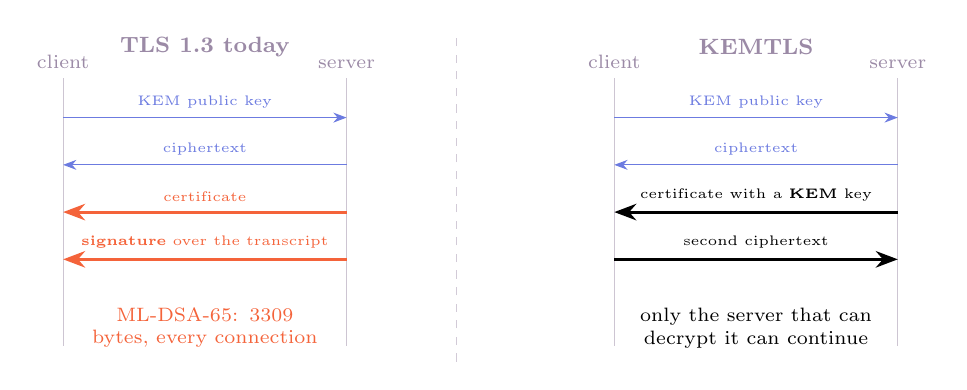
\begin{tikzpicture}[font=\scriptsize,x=1cm,y=1cm]
    \node[grey,font=\footnotesize\bfseries] at (2.4,2.5) {TLS 1.3 today};
    \draw[grey!50] (0.6,2.1) -- (0.6,-1.3);
    \draw[grey!50] (4.2,2.1) -- (4.2,-1.3);
    \node[grey,anchor=south] at (0.6,2.1) {client};
    \node[grey,anchor=south] at (4.2,2.1) {server};
    \draw[-{Stealth},peri] (0.6,1.6) -- (4.2,1.6)
      node[midway,above,font=\tiny]{KEM public key};
    \draw[-{Stealth},peri] (4.2,1.0) -- (0.6,1.0)
      node[midway,above,font=\tiny]{ciphertext};
    \draw[-{Stealth},bad,line width=1.1pt] (4.2,0.4) -- (0.6,0.4)
      node[midway,above,font=\tiny,bad]{certificate};
    \draw[-{Stealth},bad,line width=1.1pt] (4.2,-0.2) -- (0.6,-0.2)
      node[midway,above,font=\tiny,bad]{\textbf{signature} over the transcript};
    \node[bad,anchor=north,align=center,text width=4cm] at (2.4,-0.7)
      {ML-DSA-65: 3309 bytes, every connection};

    \draw[grey!45,dashed] (5.6,-1.5) -- (5.6,2.7);

    \node[grey,font=\footnotesize\bfseries] at (9.4,2.5) {KEMTLS};
    \draw[grey!50] (7.6,2.1) -- (7.6,-1.3);
    \draw[grey!50] (11.2,2.1) -- (11.2,-1.3);
    \node[grey,anchor=south] at (7.6,2.1) {client};
    \node[grey,anchor=south] at (11.2,2.1) {server};
    \draw[-{Stealth},peri] (7.6,1.6) -- (11.2,1.6)
      node[midway,above,font=\tiny]{KEM public key};
    \draw[-{Stealth},peri] (11.2,1.0) -- (7.6,1.0)
      node[midway,above,font=\tiny]{ciphertext};
    \draw[-{Stealth},good,line width=1.1pt] (11.2,0.4) -- (7.6,0.4)
      node[midway,above,font=\tiny,good]{certificate with a \textbf{KEM} key};
    \draw[-{Stealth},good,line width=1.1pt] (7.6,-0.2) -- (11.2,-0.2)
      node[midway,above,font=\tiny,good]{second ciphertext};
    \node[good,anchor=north,align=center,text width=4.4cm] at (9.4,-0.7)
      {only the server that can decrypt it can continue};
  \end{tikzpicture}
  \vspace{1mm}
  \begin{itemize}\footnotesize
    \item<2-> The handshake signature disappears. Proving you can
      decrypt is proof enough, and ML-KEM is smaller than any
      post-quantum signature.
    \item<3-> Price: authentication is \alert{implicit} at first, and
      the server's first data waits one extra flight.
    \item<4-> \cgrey{The CA still signs your certificate. KEMTLS
      removes the one signature made live; Merkle tree certificates
      remove the four made in advance.}
  \end{itemize}
\end{frame}

\begin{frame}{The escape hatch nobody wants: symmetric all the way down}
  \centering
  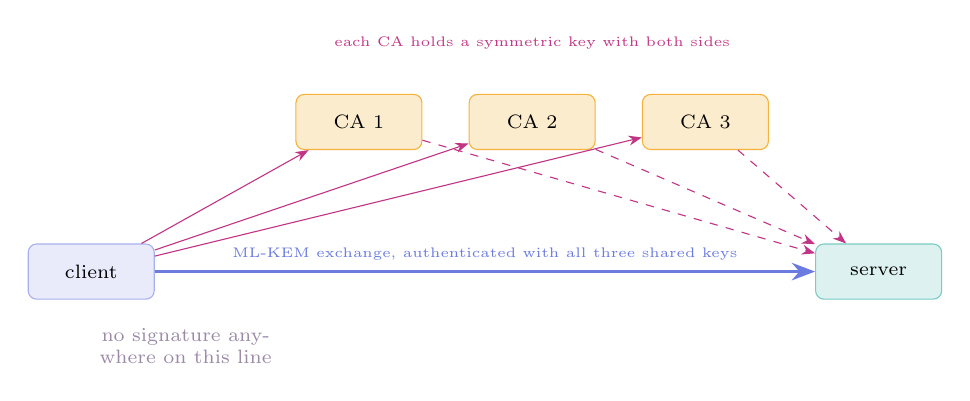
\begin{tikzpicture}[font=\scriptsize,x=1cm,y=1cm,
      b/.style={rounded corners=3pt,inner sep=5pt,minimum width=16mm,
                minimum height=7mm,line width=0.4pt}]
    \node[b,fill=peri!15,draw=peri!60] (cl) at (0,0) {client};
    \node[b,fill=good!15,draw=good!60] (sv) at (10,0) {server};
    \node[b,fill=warm!25,draw=warm] (ca1) at (3.4,1.9) {CA 1};
    \node[b,fill=warm!25,draw=warm] (ca2) at (5.6,1.9) {CA 2};
    \node[b,fill=warm!25,draw=warm] (ca3) at (7.8,1.9) {CA 3};
    \foreach \c in {ca1,ca2,ca3}{
      \draw[-{Stealth},acc] (cl) -- (\c);
      \draw[-{Stealth},acc,dashed] (\c) -- (sv);}
    \draw[-{Stealth},peri,line width=1.2pt] (cl) -- (sv)
      node[midway,above,font=\tiny,peri]{ML-KEM exchange, authenticated
        with all three shared keys};
    \node[grey,anchor=north,align=center,text width=3.4cm] at (1.2,-0.6)
      {no signature anywhere on this line};
    \node[acc,anchor=south,font=\tiny] at (5.6,2.7)
      {each CA holds a symmetric key with both sides};
  \end{tikzpicture}
  \vspace{2mm}
  \begin{itemize}\footnotesize
    \item<2-> The server's DNS carries a key per CA, encrypted to that
      CA and bound to the hostname. The client asks three CAs to pass
      a fresh key through. Symmetric throughout, already
      post-quantum.
    \item<3-> \alert{Three CAs must collude} for an attack.
    \item<4-> every CA
      learns which sites you visit, live. Like OCSP, but worse. \\ \pause
     \cgrey{Adam Langley, \url{https://www.imperialviolet.org/2024/04/07/letskerberos.html}}
  \end{itemize}
\end{frame}
          % ---------------------------------------------------------------------
          \begin{frame}{Her walk, in hindsight}
            \centering
            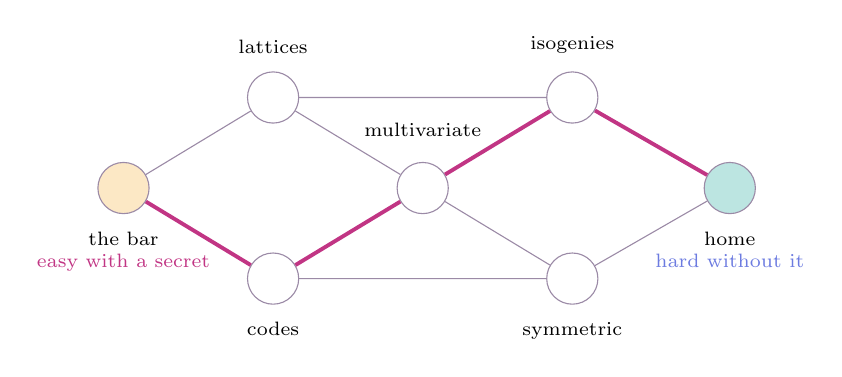
\begin{tikzpicture}[font=\scriptsize,
              v/.style={circle,draw=grey,fill=white,minimum size=6.5mm,inner sep=0},
              lab/.style={font=\scriptsize,align=center}]
              \node[v,fill=warm!30] (s) at (0,0) {};
              \node[v] (a) at (1.9,1.15) {};
              \node[v] (b) at (1.9,-1.15) {};
              \node[v] (c) at (3.8,0) {};
              \node[v] (d) at (5.7,1.15) {};
              \node[v] (e) at (5.7,-1.15) {};
              \node[v,fill=good!30] (h) at (7.7,0) {};
              \draw[grey] (s)--(a) (s)--(b) (a)--(c) (b)--(c) (c)--(d) (c)--(e)
              (d)--(h) (e)--(h) (a)--(d) (b)--(e);
              \draw[acc,line width=1.4pt] (s)--(b)--(c)--(d)--(h);
              \node[lab,below=1mm of s] {the bar\\ \cacc{easy with a secret}};
              \node[lab,above=1mm of a] {lattices};
              \node[lab,below=1mm of b] {codes};
              \node[lab,above=1mm of c,yshift=1mm] {multivariate};
              \node[lab,above=1mm of d] {isogenies};
              \node[lab,below=1mm of e] {symmetric};
              \node[lab,below=1mm of h] {home\\ \cgood{hard without it}};
            \end{tikzpicture}
            \vfill
            \begin{center}
              \alert{Where do we go?}
            \end{center}
          \end{frame}

          % ---------------------------------------------------------------------

          \heroframe{
            \node[builder,hero,shirt=teal] (d) {};
            \begin{scope}[shift={(2.0,-0.35)},scale=0.9]
              \fill[white,draw=grey,thick,rounded corners=2pt] (0,0) rectangle (1.0,1.35);
              \fill[grey!40] (0.25,1.25) rectangle (0.75,1.45);
              \foreach \y in {0.25,0.55,0.85}{\draw[grey] (0.15,\y) -- (0.85,\y);}
          \end{scope}}
          {the Deployer}{The ethical stage: commiting to an algorithm}


          \begin{frame}{The whole menu}
  \centering\footnotesize
  \begin{tabular}{@{}l l l@{}}
    \toprule
    \textbf{standard} & \textbf{what it is} & \textbf{status} \\
    \midrule
    ML-KEM (FIPS 203) & key exchange, lattices & \cgood{shipping, everywhere} \\
    ML-DSA (FIPS 204) & signatures, lattices & \cgood{the default} \\
    SLH-DSA (FIPS 205) & signatures, hashes & \cgood{slow, conservative} \\
    LMS / XMSS (SP 800-208) & signatures, hashes, stateful & \cgood{firmware} \\
    FN-DSA (FIPS 206) & signatures, lattices, small & \cwarm{still draft} \\
    HQC & key exchange, codes & \cwarm{backup, picked 2025} \\
    \bottomrule
  \end{tabular}
  \vspace{3mm}
  \begin{itemize}
    \item<2-> That is the list. Six things, two of which nobody ships
      yet.
    \item<3-> Everything else is either research
      prototype or in standardization process
  \end{itemize}
\end{frame}

\begin{frame}{Nobody asked you}
  \begin{itemize}
    \item<1-> The internet has decided. Browsers, OpenSSL, Go, Apple,
      the big CDNs: post-quantum key exchange is on by default and
      the share only goes up.
    \item<2->  the question is \emph{when} rather than \emph{whether}.
    \item<3-> \alert{Betting against a decade of coordinated
      engineering effort is usually a bad bet.} 
  \end{itemize}
\end{frame}

\begin{frame}{``But it is bigger''}
  \centering
  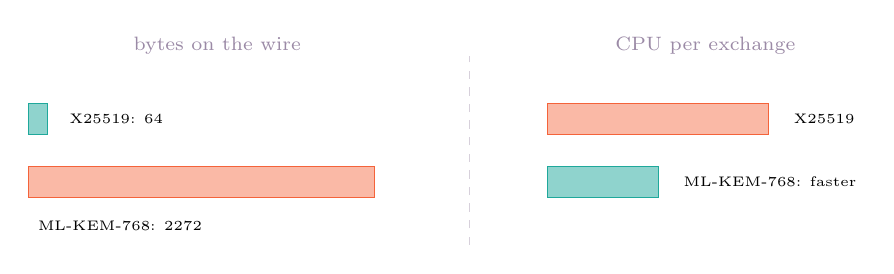
\begin{tikzpicture}[font=\scriptsize,x=1cm,y=1cm]
    \node[grey,anchor=south] at (2.4,2.5) {bytes on the wire};
    \fill[good!50,draw=good] (0,1.6) rectangle (0.25,2.0);
    \node[anchor=west,font=\tiny] at (0.4,1.8) {X25519: 64};
    \fill[bad!45,draw=bad] (0,0.8) rectangle (4.4,1.2);
    \node[anchor=west,font=\tiny] at (0,0.45) {ML-KEM-768: 2272};

    \draw[grey!40,dashed] (5.6,0.2) -- (5.6,2.6);

    \node[grey,anchor=south] at (8.6,2.5) {CPU per exchange};
    \fill[bad!45,draw=bad] (6.6,1.6) rectangle (9.4,2.0);
    \node[anchor=west,font=\tiny] at (9.6,1.8) {X25519};
    \fill[good!50,draw=good] (6.6,0.8) rectangle (8.0,1.2);
    \node[anchor=west,font=\tiny] at (8.2,1.0) {ML-KEM-768: faster};
  \end{tikzpicture}
  \vspace{3mm}
  \begin{itemize}
    \item<2-> Lattices are bigger, but \alert{faster} than elliptic curves.
    \item<3-> bytes are in the hot path of every connection, including  a bad mobile link
    \item<4-> Though if you ship an Electron app, you have
      forfeited the right to complain about two kilobytes.
  \end{itemize}
\end{frame}
%               % ---------------------------------------------------------------------
%           \begin{frame}{A choice of algorithms}
%             \centering\footnotesize
%             \begin{tabular}{@{}l p{3.0cm} p{3.4cm} p{3.6cm}@{}}
%              \toprule
%     & \textbf{shipping} & \textbf{candidate} & \textbf{cryptanalysis summer} \\
%     \midrule
%               lattices     & ML-KEM, ML-DSA, Falcon & HAWK & \cbad{HAWK is a non-starter} \\[2pt]
%               symmetric    & SLH-DSA, LMS/XMSS & FAEST, MQOM, SDitH & \cgood{boring, sturdy} \\[2pt]
%               codes        & HQC & \cgrey{nothing left} & \cgrey{keys the size of a photo} \\[2pt]
%               multivariate & \cgrey{none} & UOV, MAYO, SNOVA, QR-UOV & \cwarm{tiny signatures, tense} \\[2pt]
%               isogenies    & \cgrey{none} & SQIsign & \cwarm{beautiful, unhurried} \\[2pt]
%               lattices, again & \cgrey{FHE exists} & & \cbad{not shippable, and I like it} \\
%               \bottomrule
%             \end{tabular}
%             \vfill
%             \vspace{2mm}
%             \footnotesize\cgrey{NIST IR 8610, second-round report: FAEST, HAWK,
%             MAYO, MQOM, QR-UOV, SDitH, SNOVA, SQIsign, UOV.}
%           \end{frame}
% 
%           % ---------------------------------------------------------------------
%           \begin{frame}{What it costs you, in bytes}
%             \centering
%             \begin{tikzpicture}[font=\scriptsize]
%               \begin{axis}[
%                 width=0.86\textwidth,height=5.0cm,
%                 xbar, xmode=log, xmin=60, xmax=600000,
%                 xlabel={public key $+$ signature, or key $+$ ciphertext},
%                 symbolic y coords={UOV,SLH-DSA,ML-DSA-65,ML-KEM-768,Falcon-512,
%                 SQIsign,ECDSA},
%                 ytick={UOV,SLH-DSA,ML-DSA-65,ML-KEM-768,Falcon-512,SQIsign,ECDSA},
%                 every axis plot/.append style={bar shift=0pt},
%                 nodes near coords,
%                 nodes near coords align={horizontal},
%                 point meta=explicit symbolic,
%                 bar width=3.6mm, enlarge y limits=0.13,
%                 every node near coord/.append style={font=\tiny},
%                 xtick={100,1000,10000,100000}, xticklabels={100,1k,10k,100k},
%                 grid=major, grid style={grey!20}]
%                 \addplot[fill=warm!70,draw=warm]  coordinates {(44100,UOV) [44100]};
%                 \addplot[fill=good!60,draw=good]  coordinates {(7888,SLH-DSA) [7888]};
%                 \addplot[fill=acc!70,draw=acc]    coordinates {(5261,ML-DSA-65) [5261]};
%                 \addplot[fill=acc!45,draw=acc]    coordinates {(2272,ML-KEM-768) [2272]};
%                 \addplot[fill=acc!25,draw=acc]    coordinates {(1563,Falcon-512) [1563]};
%                 \addplot[fill=bad!45,draw=bad]    coordinates {(213,SQIsign) [213]};
%                 \addplot[fill=grey!45,draw=grey]  coordinates {(128,ECDSA) [128]};
%               \end{axis}
%             \end{tikzpicture}
%             \vfill
%             \begin{tabular}{@{}l l l@{}}
%     \toprule
%     \textbf{NIST PQC level} & \textbf{at least as hard as} & \textbf{examples} \\
%     \midrule
%     1 & recovering an AES-128 key & ML-KEM-512, SLH-DSA-128s \\
%     2 & finding a SHA-256 collision & ML-DSA-44 \\
%     3 & recovering an AES-192 key & ML-KEM-768, ML-DSA-65 \\
%     4 & finding a SHA-384 collision & \cgrey{---} \\
%     5 & recovering an AES-256 key & ML-KEM-1024, ML-DSA-87 \\
%     \bottomrule
%   \end{tabular}
% 
%           \end{frame}
% 

\begin{frame}{The state of the post-quantum internet}
  \centering
  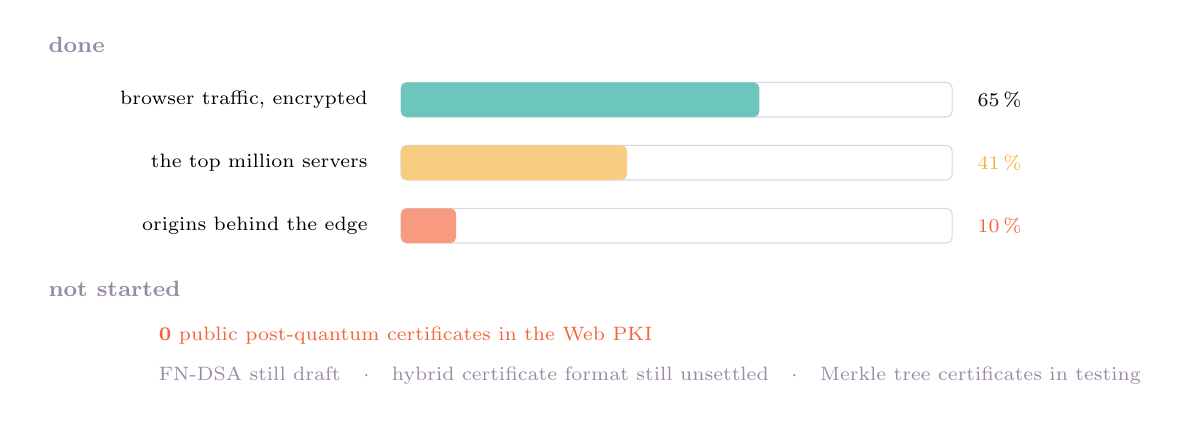
\begin{tikzpicture}[font=\scriptsize,x=1cm,y=1cm]
    \node[grey,anchor=west,font=\footnotesize\bfseries] at (-4.6,2.4) {done};
    \foreach \y/\lab/\val/\col in {%
      1.7/{browser traffic, encrypted}/65/good,
      0.9/{the top million servers}/41/warm,
      0.1/{origins behind the edge}/10/bad}{
      \node[anchor=east,align=right,text width=4.2cm] at (-0.3,\y) {\lab};
      \draw[grey!35,rounded corners=2pt] (0,\y-0.22) rectangle (7,\y+0.22);
      \fill[\col!65,rounded corners=2pt] (0,\y-0.22) rectangle (0.07*\val,\y+0.22);
      \node[anchor=west,\col] at (7.2,\y) {\val\,\%};}
    \node[grey,anchor=west,font=\footnotesize\bfseries] at (-4.6,-0.7) {not started};
    \node[anchor=west,bad,align=left] at (-3.2,-1.3)
      {\textbf{0} public post-quantum certificates in the Web PKI};
    \node[anchor=west,grey,align=left] at (-3.2,-1.8)
      {FN-DSA still draft \ \ $\cdot$ \ \ hybrid certificate format still
       unsettled \ \ $\cdot$ \ \ Merkle tree certificates in testing};
  \end{tikzpicture}
  \vspace{1mm}
  \begin{itemize}\footnotesize
    \item<2-> Encryption is nearly done. It took ten years, most middleboxes, not mathematics.
    \item<3-> \alert{Authentication has not started.} Not one
      publicly trusted certificate uses a post-quantum signature.
    \item<4-> \cgrey{Cloudflare and Tranco scans, mid-2026.}
  \end{itemize}
\end{frame}

          \begin{frame}[standout]
            If it can be broken, it can be fixed. 
          \end{frame}

          % ---------------------------------------------------------------------
          \begin{frame}{Merkle Tree Certificates}
  \centering
  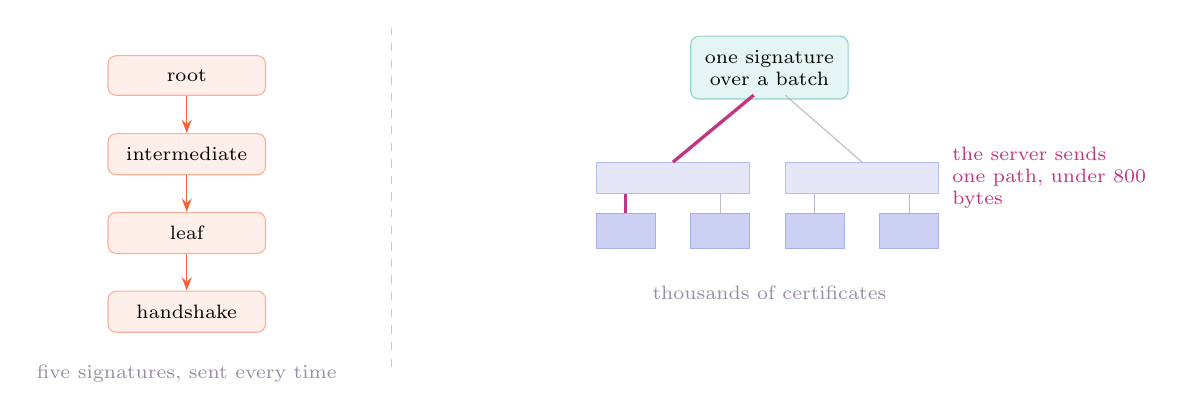
\begin{tikzpicture}[font=\scriptsize,x=1cm,y=1cm,
      b/.style={rounded corners=3pt,inner sep=5pt,align=center,
                line width=0.4pt,minimum width=20mm}]
    % today
    \node[b,fill=bad!10,draw=bad!50] (r1) at (0,1.6) {root};
    \node[b,fill=bad!10,draw=bad!50] (i1) at (0,0.6) {intermediate};
    \node[b,fill=bad!10,draw=bad!50] (l1) at (0,-0.4) {leaf};
    \node[b,fill=bad!10,draw=bad!50] (h1) at (0,-1.4) {handshake};
    \draw[-{Stealth},bad] (r1)--(i1); \draw[-{Stealth},bad] (i1)--(l1);
    \draw[-{Stealth},bad] (l1)--(h1);
    \node[grey,anchor=north] at (0,-1.95) {five signatures, sent every time};

    \draw[grey!50,dashed] (2.6,-2.1) -- (2.6,2.2);

    % with MTC
    \node[b,fill=good!12,draw=good!50] (sig) at (7.4,1.7) {one signature\\ over a batch};
    \foreach \x in {5.2,6.4,7.6,8.8}{
      \fill[peri!35,draw=peri!60] (\x,-0.6) rectangle ++(0.75,0.45);}
    \foreach \x/\y in {5.575/0.1,6.775/0.1,7.975/0.1,9.175/0.1}{
      \draw[grey!60] (\x,-0.15) -- (\x,\y);}
    \foreach \x in {5.2,7.6}{
      \fill[peri!18,draw=peri!50] (\x,0.1) rectangle ++(1.95,0.4);}
    \draw[grey!60] (6.175,0.5) -- (7.2,1.35);
    \draw[grey!60] (8.575,0.5) -- (7.6,1.35);
    \draw[acc,line width=1.2pt] (5.575,-0.15) -- (5.575,0.1);
    \draw[acc,line width=1.2pt] (6.175,0.5) -- (7.2,1.35);
    \node[acc,anchor=west,align=left,text width=2.5cm] at (9.6,0.3)
      {the server sends one path, under 800 bytes};
    \node[grey,anchor=north] at (7.4,-0.95) {thousands of certificates};
  \end{tikzpicture}
  \begin{itemize}\small
    \item PQ signatures are large
    \item<2-> Sign batch once, proves membership:  four of the five signatures disappear.
    \item<3-> trust moves from ``verify a chain
      now'' to ``I already know the root''.
    \item<4-> \alert{In the common case this is smaller than what we
      send today}, so post-quantum authentication could end up faster
      than classical.
  \end{itemize}
  \vfill
  \footnotesize\cgrey{X.509 stays: for clients without the root, for
  anything outside a batch, and as the fallback. It just stops being
  on the hot path.}
\end{frame}

          % ---------------------------------------------------------------------
          \begin{frame}{When does a useful quantum computer arrive?}
            \begin{itemize}
              \item Estimates run from the early 2030s to the mid-2040s.
              \item A lot of arguments: Hybrids, key sizes, which curve to keep\pause
              \item Transition is as soon as 2029 (Google, Cloudflare)
            \end{itemize}
          \end{frame}

          % =====================================================================

          \heroframe{\node[graduate,hero,female,shirt=blush] {};}
          {the Academic}{What is to be done?}

          \begin{frame}{Privacy gets more difficult}
  \centering
            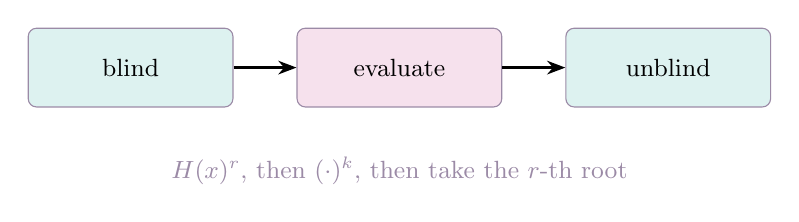
\begin{tikzpicture}[font=\small,node distance=8mm,
              b/.style={draw=grey,rounded corners=3pt,fill=white,minimum height=10mm,
              minimum width=26mm,align=center}]
              \node[b,fill=good!15] (bl) {blind};
              \node[b,right=of bl,fill=acc!15] (ev) {evaluate};
              \node[b,right=of ev,fill=good!15] (un) {unblind};
              \draw[-{Stealth},thick] (bl)--(ev); \draw[-{Stealth},thick] (ev)--(un);
              \node[below=5mm of ev,font=\small,grey]
                {$H(x)^{r}$, then $(\cdot)^{k}$, then take the $r$-th root};
            \end{tikzpicture}
  \begin{itemize}
    \item exact,
      leak-free blinding: Kuperberg  \pause
\item Need to slap on a lot of zero-knowledge proofs, counting arguments
  \end{itemize}

          \end{frame}

          \begin{frame}{Cryptanalysis summer}
  \begin{itemize}
    \item \cbad{HAWK fell} to a classical attack. \pause\\ Used structure other lattices didn't have.
    \item \cgood{A quantum algorithm claimed the dihedral coset
      problem in polynomial time.} \pause\\ 
      Actually strengthened lattices: conjecture
      that whole families of quantum lattice attacks may never gain
      more than a polynomial factor. 
    \item<3-> \cbad{Classic McEliece got a distinguisher}, which
      became a quasi-polynomial key recovery. Nobody has run it, much
      like RSA-1024.   \end{itemize}
  \vfill
\end{frame}

          % ---------------------------------------------------------------------
          \begin{frame}{Building to break}
            \centering
            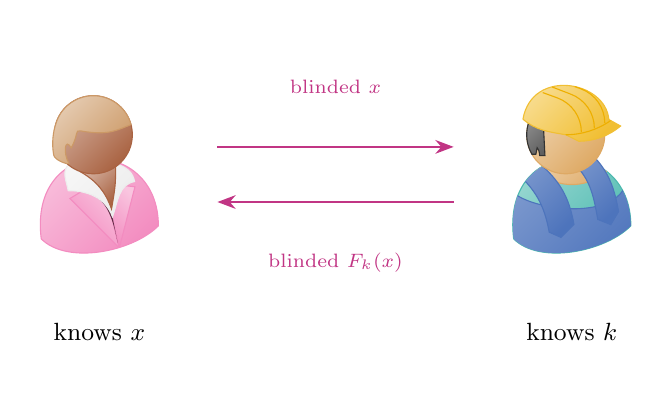
\begin{tikzpicture}[every node/.style={minimum size=1.5cm},font=\small]
              \node[alice,shirt=rose,hair=brown,label=below:{knows $x$}] (a) at (0,0) {};
              \node[builder,shirt=teal,label=below:{knows $k$}] (s) at (6,0) {};
              \draw[-{Stealth},acc,thick] (1.5,0.35) -- (4.5,0.35)
                node[midway,above,font=\scriptsize]{blinded $x$};
              \draw[{Stealth}-,acc,thick] (1.5,-0.35) -- (4.5,-0.35)
                node[midway,below,font=\scriptsize]{blinded $F_k(x)$};
            \end{tikzpicture}
            \vfill
            \begin{itemize}
              \item She learns $F_k(x)$. He learns nothing. Neither learns the
                other's secret.
              \item ``Is my password in this breach?'' without saying the
                password. Private contact discovery. Anonymous tokens.
              \item As an instrument: the smallest protocol that  shows
                whether a primitive is \alert{flexible}.
            \end{itemize}
          \end{frame}

    %       % ---------------------------------------------------------------------
    %       \begin{frame}{The property I keep wanting and cannot have}
    %         \begin{alertblock}{Random self-reducibility}
    %           Any single hard instance can be re-randomised into a fresh random
    %           one. So one instance is as hard as the average, and I can blind
    %           with no loss.
    %         \end{alertblock}
    %         \vfill
    %         \begin{itemize}
    %           \item Learning with errors has this, by way of a worst-case to
    %             average-case reduction. That is what makes it beloved.
    %           \item But every re-randomisation adds fresh noise, and I need the
    %             protocol to be \alert{deterministic}: both sides must land on
    %             the same output, every time.
    %           \item Deterministic pushes me to rounding instead of noise:
    %             learning with rounding, which behaves, and gives up the
    %             reduction that made me comfortable in the first place.
    %         \end{itemize}
    %       \end{frame}

              \begin{frame}{What now? }
  \centering
  
\begin{tikzpicture}[every node/.style={minimum size=1.5cm}]
    \node[chef,female,shirt=black, details=pink!70!white,hat=black,hair=pink] at (0,0)   {};
    \node[alice,    shirt=mauve,hair=brown,] at (2.6,0) {};
    \node[builder,  shirt=teal] at (5.2,0) {};
    \node[graduate, shirt=blush] at (7.8,0) {};
  \end{tikzpicture}
  \vspace{4mm}

  \begin{minipage}{0.86\textwidth}
    \onslide<2->{\large We choose without knowing, which Kierkegaard
      said is the only kind of choosing there is.\par}
    \vspace{3mm}
    \onslide<3->{\large \cacc{I am afraid we will lose privacy on the
      way}, because the tools that protect it are the ones that do not
      survive the move.\par}
    \vspace{3mm}
    \onslide<4->{\large And still: the mathematics is beautiful, we get
      to open systems nobody has opened in thirty years, and almost
      none of it is decided yet.\par}
  \end{minipage}
\end{frame}

\begin{frame}[standout]
  Stop being sad.\\[5mm]
  {\normalsize Break something. On a laptop. Over a weekend.}
\end{frame}

\begin{frame}{References}
  \centering
  \begin{itemize}
    \item Sophie Schmieg's blog, especially \url{keymaterial.net/2025/12/13/a-very-unscientific-guide-to-the-security-of-various-pqc-algorithms/}
  \item Security Cryptography Whatever, especially \url{https://securitycryptographywhatever.com/2026/08/26/ai-lattice-proofs-with-chris-peikert/}
  \item Bas Westerbaan's blog, especially 
\end{itemize}
\end{frame}

          % ---------------------------------------------------------------------
          \begin{frame}[standout]
            Thank you.\\[4mm]
            {\normalsize heimberger.xyz}
          \end{frame}

          \end{document}
